\chapter{Харчаваньне}

\section{Харчаваньне як аснова здароўя}

«Няхай ваша ежа будзе вашым лекамі, інакш лекі стануць вашай ежай»,~--- сказаў Гіпакрат яшчэ прыкладна ў~IV стагодзьдзі да н.э. Мы ямо некалькі разоў кожны дзень~--- гэта самае частае зь дзеяньняў, што мы ажыцьцяўляем і якое значна ўплывае на наша здароўе. 

Харчаваньне знаходзіцца пад нашым кантролем: мы самі вызначаем, што менавіта і ў~якой колькасьці трапіць да нас на талерку і як мы гэта зьямо. Невыпадкова шлях да зьмены ладу жыцьця для большасьці людзей пачынаецца менавіта з~харчаваньня. І вы здольныя вырашыць многія пытаньні са здароўем відэльцам, пакуль гэта не зрабіў хірург скальпелем. 

\textbf{Мой курс здаровага харчаваньня~--- самы папулярны ў~параўнаньні з~курсамі іншых рэсурсаў здароўя. Здаровае харчаваньне павінна быць зручным для вас, сынхранізаванае з~вашым ладам жыцьця і не зьяўляцца прычынай дыскамфорту і абмежаваньняў.} 

\infobox{Памятайце, што мы ямо, каб жыць, а~не жывём, каб есьці!}

Нават невялікія зьмены ў~харчаваньні на працягу доўгага часу здольныя даць магутны станоўчы эфэкт. Павысіўшы ўсьвядомленасьць спачатку ў~ежы, далей мы можам па аналёгіі распаўсюдзіць усьвядомленае стаўленьне і на іншыя аспэкты: напрыклад, задумацца аб тым, якую ежу атрымлівае наш мозг ад камунікацыі і сацсетак. Харчаваньне зьяўляецца ключавой звычкай, яно трэніруе ўвагу і вучыць рабіць выбар сьвядома, а~не пад уплывам інстынктаў ці асяродзьдзя.

Рэжым харчаваньня, тыпы прадуктаў і колькасьць ежы ўплываюць на працу гармонаў і адчувальнасьць арганізма да іх, што, у~сваю чаргу, уплывае на мэтабалізм, выпрацоўку энэргіі ў~мітахондрыях, зьмену актыўнасьці генаў, глыбіню сну, трывушчасьць, лібіда\index{лібіда}, разумовыя здольнасьці, працягласьць жыцьця і вонкавы выгляд. Навукоўцы сёньня ўжо адмовіліся ад ацэнак харчаваньня па наяўнасьці ў~дыеце тых ці іншых прадуктаў, а~вывучаюць харчовыя патэрны цалкам, то бок поўны набор прадуктаў, якія вы ясьце, частасьць іх спажываньня, рэжым харчаваньня, колькасьць зьедзенага.

У гэтым разьдзеле мы будзем абмяркоўваць самыя розныя аспэкты харчаваньня і адкажам на пытаньні: 

\begin{itemize}
  \item \textbf{калі есьці?}~--- пра рэжым харчаваньня,
  \item \textbf{як есьці?}~--- пра яду,
  \item \textbf{што есьці?}~--- пра прадукты,
  \item \textbf{колькі есьці?}~--- як балянсаваць свой каляраж.
\end{itemize}

\subsection*{Харчовая матрыца}
Фройд лічыў, што сьветам кіруе сэксуальны інстынкт, але першасным зьяўляецца менавіта харчовы інстынкт. Галодным не да сэксу, а~галаданьне зьніжае і лібіда\index{лібіда}, і ўзровень палавых гармонаў. Звычкі, якія мы разьвіваем падчас яды, могуць быць перанесеныя і на іншыя сфэры жыцьця. 

\infobox{Усьвядомленасьць зараджаецца як увага да ежы на сваёй талерцы, таму кожны прыём ежы можна ператварыць у~мэдытацыю\index{мэдытацыя}.}

Уменьне актыўна ўзаемадзейнічаць зь ежай, калі мы старанна кусаем і разжоўваем яе,~--- гэта база для таго, каб «грызьці граніт навукі» або «ўрваць свой кавалак па жыцьці», а~не заставацца «сысунком». Харчаваньне можа разьвіць наш густ так, што мы навучымся атрымліваць задавальненьне ад складанай ежы і смакаў, а~ня проста бамбаваць свае рэцэптары вульгарнымі тлуста-салодка-смажана-салёнымі спалучэньнямі.

\emph{Тое, як мы ставімся да ежы, праецыруецца і на нашае стаўленьне да жыцьця наогул. Таму для таго, каб скласьці ўяўленьне пра чалавека, убачыць яго сапраўднага, паабедайце з~ім. Тое, як ён есьць, як абыходзіцца зь ежай, як жуе, як пачынае і заканчвае сталаваньне, шмат скажа пра яго асобу.}

\begin{figure}[htb!]
  \centering
  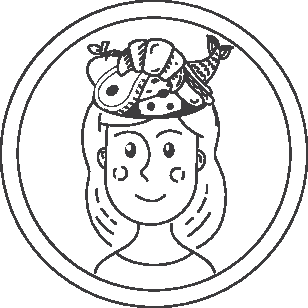
\includegraphics[scale=1.5]{willpower/ch4/1.pdf}
\end{figure}

\textbf{«Ты~--- гэта тое, што ты ясі»~---} і мы разумеем важнасьць якаснага складу ежы. «Калі ты ясі, колькі трэба, ты корміш цела. А тым, што пераядаеш, ты корміш хваробы»,~--- старажытныя і мудрыя казалі так. Сёньня мы таксама разумеем, што важная таксама колькасьць спажыванай ежы. Харчаваньне можа як павялічваць рызыкі шматлікіх захворваньняў, так і зьмяншаць іх.

\emph{Няма, бадай, такой хваробы, цячэньне якой так ці інакш не было б зьвязанае з~харчаваньнем, акрамя, мабыць, траўмаў. Хоць і траўмы магчымыя, калі вы ясьце на хаду і пасьлізгваецеся на роўным месцы.}

Харчаваньне~--- адзін з~галоўных рэсурсаў здароўя, і гэты рэсурс да краёў запоўнены няслушнай інфармацыяй, мітамі і супрацьлеглымі меркаваньнямі. У гэтай тэме багата адмыслоўцаў, інста-гуру і аўтараў, якія прапануюць сумнеўныя і адкрыта небясьпечныя мэтодыкі «аздараўленьня». Часта ў~іх маецца акцэнт толькі на адным з~аспэктаў харчаваньня: нехта змагаецца зь бялком, іншыя~--- з~вугляводамі, трэція~--- з~тлушчамі, чацьвёртыя прапануюць то закісьляць, то зашчолваць, пятыя вядуць вайну з~глютэнам і да т.~п. Многія людзі ў~выніку такой «адукацыі» ставяцца да ежы спрошчана: галоўным крытэрам становіцца, напрыклад, колькасьць калёрыяў ці адпаведнасьць ежы нейкім пунктам~--- арганічная, безглютэнавая ці да т.~п.

\infobox{«Карысная ежа» таксама можа быць нездаровай або разрэклямаванай: у~розныя пэрыяды карыснымі лічыліся маргарын, фруктоза, сокі, абястлушчаныя прадукты. Цяпер можна бачыць, як штогод зьяўляюцца свае «модныя» карысныя прадукты, то пік папулярнасьці хлярэлы, то годжы, то сьпіруліны, то чыа.}

\emph{Мы з~вамі назіралі і фанатычнае змаганьне з~тлушчамі, калі іх абвясьцілі галоўнай прычынай сардэчна-сасудзістых захворваньняў\index{сардэчна-сасудзістыя захворваньні}, а~затым, калі гэта не пацьвердзілася, хвалю захапленьня кета-дыетай. Зь бялкамі дакладна такая ж гісторыя~--- спачатку жывёльныя бялкі дэманізаваліся і ўсе хацелі стаць вэганамі, затым модным стаў карнівор, калі ядуць толькі ежу жывёльнага паходжаньня, а~расьлінная абвяшчаецца шкоднай. У моду ўваходзяць то доўгія галадоўкі, то дробавае харчаваньне, то захапленьне дэтоксамі на фруктовых соках, то спробы замяніць паўнавартаснае харчаваньне наборам БАДаў. Усе гэтыя скрайнасьці як мінімум некарысныя, як максімум~--- небясьпечныя.}

\infobox{Акрамя фізычнае шкоды, зацыкленасьць на харчаваньні можа прыводзіць і да разладаў харчовых паводзінаў: анарэксіі\index{анарэксія} і буліміі. Ёсьць і яшчэ не прызнаныя навукай парушэньні, напрыклад артарэксія\index{артарэксія}~--- фіксацыя на правільным харчаваньні.} 

\textbf{Артарэксік упэўнены, што толькі яго харчаваньне правільнае і ён сам «правільны», а~ўсё вакол~--- «няправільныя» і ядуць няправільную ежу. Гэтае парушэньне суправаджаецца нецярпімасьцю да поглядаў іншых людзей на здароўе і, як вынік, прыводзіць да ізаляцыі.}

Шкада, што ежа замест задавальненьня фізычнага голаду робіцца сродкам самасьцьвярджэньня. У выпадку здаровага харчаваньня чалавек імкнецца выпрацаваць аптымальную, зручную, гнуткую стратэгію харчаваньня, якая нясе задаволенасьць і карысьць ды пасуе менавіта яму; тады чалавек разумее, што яго стратэгія пасавацьме ня кожнаму і адаптаваная выключна індывідуальна~--- пад асаблівасьці арганізма і рэжым дня.

Нягледзячы на тое, што ў~сьвеце расьце разуменьне важнасьці здаровага харчаваньня, колькасьць выпадкаў атлусьценьня\index{атлусьценьне} працягвае павялічвацца. Зьмяніць харчаваньне досыць складана~--- гэта ж найважнейшы чыньнік выжываньня, таму пры спробах паменшыць колькасьць спажыванай ежы або зьмяніць тыя ці іншыя перавагі нашая біялёгія можа працаваць супраць нас. 

\emph{Як у~анекдоце: ад адной думкі пра дыету на мяне нападае шалёны апэтыт.}

\textbf{Улічвайце індывідуальныя асаблівасьці.} Мы ўсе розныя генэтычна, вядзём розны лад жыцьця, маем розную мікрафлёру, таму складаньне індывідуальнай ідэальнай дыеты патрабуе пэрсаналізацыі ўсіх рэкамэндацыяў. Кожны прадукт мае свае станоўчыя і адмоўныя бакі, гэта залежыць і ад кантэксту дыеты, і ад колькасьці зьедзенага. Ёсьць розьніца паміж дададзеным цукрам і цукрам у~цэльным фрукце, паміж смажанай рыбай з~салодкім соусам і прыгатаванай на пары, паміж рыбай дзікае лоўлі і дадаткам рыбінага тлушчу.

\emph{Часам дзеяньне прадукту вызначаецца мікрафлёрай. Так, пры ўжываньні граната ўтварэньне ў~кішачніку карыснага для здароўя рэчыва уралітыну залежыць ад наяўнасьці пэўных бактэрыяў, гэтак жа, як і ўтварэньне шкоднага трымэтылямін-аксіду пры спажываньні яек. Кафэін можа як падвышаць, так і зьмяншаць сыстэмнае запаленьне, поліненасычаныя тлустыя кіслоты могуць як падвышаць, так і зьмяншаць узровень добрага халестэрыну ў~залежнасьці ад індывідуальнай генэтыкі. На глікемічны індэкс уплывае вага чалавека, узрост, мікрафлёра, прыём ежы да гэтага і нават выспаўся ён ці не.}

«Я пачаў займацца спортам і правільна харчавацца, але не схуднеў. Відаць, таму, што не перастаў хлусіць сабе». Самы просты спосаб узяць харчаваньне пад кантроль~--- \textbf{гэта вядзеньне харчовага дзёньніка.} Калі складана рабіць гэта кожны дзень, то можаце проста фатаграфаваць прыём ежы перад ядой, а~затым раз на тыдзень праводзіць рэвізію свайго рацыёну па здымках. Харчовы дзёньнік паляпшае дысцыпліну, аўтаматычна стымулюе вас рабіць больш здаровы выбар, заўважаць рэакцыю арганізма на тыя ці іншыя прадукты. Харчовы дзёньнік таксама дазволіць заўважыць прычыны адхіленьняў ад здаровага харчаваньня (недасып, стрэс і інш.). 

\emph{Карысна экспэрымэнтаваць са сваім харчаваньнем, прыбіраючы і затым дадаючы пэўныя прадукты. Элімінацыйная дыета, калі вы спачатку на тыдзень выключаеце з~рацыёну пэўны прадукт, затым уводзіце яго і назіраеце за зьменамі, дае магчымасьць заўважыць непераноснасьць ці асаблівасьці дзеяньня тых ці іншых прадуктаў на ваш стан.}

Можна правесьці ДНК-тэставаньне, якое дазваляе выявіць некаторыя непераноснасьці і асаблівасьці вашага мэтабалізму. Назіраньне за паводзінамі глюкозы з~дапамогай глюкомэтра або сыстэмы сталага маніторынгу дапамагае выявіць індывідуальныя рэакцыі на розную ежу. Дасьледаваньне мікрабіёмы кантралюе эфэктыўнасьць мерапрыемстваў, накіраваных на ўзбагачэньне рацыёну прабіётыкамі і прэбіётыкамі, павышэньне разнастайнасьці кішачнай мікрафлёры.

\subsection*{Пытаньні і заданьні}

1. Якія ў~вас ёсьць шкодныя харчовыя звычкі? А карысныя?

2. Вы паважаеце ежу ці пабойваецеся яе? Якія ў~вас адносіны?

3. Колькі разоў вы спрабавалі дыеты і як мянялася вашая вага ў~працэсе і пасьля?


\section{Уплыў на здароўе}

Назіраючы людзей з~рознымі праблемамі здароўя, я бачу, што не існуе такой хваробы ці стану, на які не магло б паўплываць паляпшэньне якасьці і рэжыму харчаваньня. 

\emph{Здаровае харчаваньне можа зьнізіць рызыку заўчаснае сьмерці на 50--60\,\%, падоўжыць жыцьцё на 8--10 гадоў, нездаровае~--- скараціць жыцьцё больш чым на 6 гадоў. Нездаровае харчаваньне болей шкоднае, чым курэньне, зьяўляючыся прамой прычынай больш за 20\,\% усіх сьмерцяў у~сьвеце і ўскоснай прычынай мноства іншых сьмерцяў. Так, ежа сапраўды становіцца вельмі эфэктыўным лекам.} 

\infobox{Сярод самых небясьпечных харчовых звычак навукоўцы лічаць дэфіцыт садавіны і гародніны, недастатковае спажываньне клятчаткі і збожжа, залішняе спажываньне солі, цукру і інш.}

На здароўе ўплываюць розныя аспэкты: напрыклад, рэжым харчаваньня, колькасьць зьедзенага, віды прадуктаў, спосабы іх гатаваньня. Рэжым харчаваньня мяркуе: колькасьць прыёмаў ежы, працягласьць харчовага вакна, час дня, калі вы ясьце. Чым меншае харчовае вакно, тым гэта карысьней для здароўя нават пры аднолькавым рацыёне. А калі зьядаць позна ўвечары багатую вячэру, то ёсьць рызыка падвышэньня ўзроўню глюкозы, а~значыць і інсуліну, і такім чынам павялічваецца рызыка дыябэту\index{дыябэт} і гіпэртэнзіі\index{гіпэртэнзія}. Чым пазьней мы вячэраем, тым вышэйшы ўзровень хранічнага запаленьня, рызыка атлусьценьня\index{атлусьценьне} і раку грудзей.

\textbf{Многія хваробы працякаюць цяжэй, калі чалавеку спадарожнічае атлусьценьне\index{атлусьценьне}.} Залішняя вага ня толькі зьяўляецца «спадарожнікам» дыябэту\index{дыябэт}, яна гэтак жа зьніжае лібіда\index{лібіда}, фэртыльнасьць, павышае ўзровень запаленьня, зьніжае таўшчыню кары галаўнога мозгу~--- нават у~падлеткаў, паскарае старэньне мозгу, павялічвае рызыку анкалягічных, сардэчна-сасудзістых, аўтаімунных захворваньняў\index{аўтаімунныя захворваньні}.

\textbf{А калі ў~вас нармальная вага?} Нават у~межах нармальнай вагі аптымізацыя структуры цела аказвае дабратворны ўплыў на здароўе. Дасьледаваньні добраахвотнікаў паказалі, што зьніжэньне каляражу ўсяго на 300 ккал у~дзень паляпшае шэраг біямаркераў, памяншаючы рызыку дыябэту, сардэчна-сасудзістых і нэўрадэгенэратыўных захворваньняў, падвышаючы лібіда і якасьць сну. Пры гэтым людзі са звычайнай вагой скінулі 10\,\% масы цела, 70\,\% зь якога складаў чысты тлушч. Худы чалавек можа мець лішні тлушч, бо вісцэральны тлушч бывае падвышаны як у~людзей з~нармальнай масай цела, так і ў~людзей з~атлусьценьнем\index{атлусьценьне}~--- падрабязьней пра гэта крыху ніжэй.

\emph{Абмежаваньне калёрыяў у~здаровых людзей зьяўляецца магутным чыньнікам падаўжэньня жыцьця. Яно паляпшае функцыю сэрца, зьніжае ўзровень інсулінападобнага чыньніка росту~--- 1 (IGF-1) і цыкляоксігеназы II (COX-2), што таксама скарачае рызыку некалькіх відаў раку. Паляпшае працу мітахондрыяў і памяншае ўзровень акісьляльнага стрэсу, павялічвае актыўнасьць ахоўных генаў, такіх як PGC-1\alpha\ і SIRT1. Важна, што як рэжым харчаваньня, так і агульная колькасьць калёрыяў могуць мадуляваць актыўнасьць mTOR~--- галоўнага кіраўніка клеткавага росту.}

\subsection*{Мінусы харчовага ўстрыманьня і абмежаваньня калёрыяў}

Значнае абмежаваньне калёрыяў зьмяншае імунітэт, узровень палавых гармонаў, можа зьмяншаць аб'ём цяглічнай масы і шчыльнасьць костак. Таму важна вызначыць для сябе аптымальнае харчаваньне бяз скрайнасьцяў. Фастынг\index{фастынг}, або інтэрвальнае галаданьне, пераносіцца лягчэй і можа быць эфэктыўным спосабам паменшыць колькасьць калёрыяў зь вялікім псыхалягічным камфортам. 

\infobox{У людзей са схільнасьцю да пераяданьня харчовыя абмежаваньні могуць справакаваць зрыў. Таму я супраць абмежавальных дыетаў: можна есьці ўсё, можна есьці заўсёды, але ня вам і ня сёньня~--- у~вас на гэтым тыдні крыху іншы плян.}

\subsection*{Раньняе старэньне} 
Уявіце, што ежа~--- гэта паліва. Чым больш і часьцей вы ясьце, тым мацней стымулюеце мэтабалічныя шляхі, як быццам ваша нага ўвесь час цісьне на пэдаль газу ў~падлогу. Але пры гэтым вы мала рухаецеся~--- гэта як быццам ваша нага адначасова цісьне й на тормаз. Такая сытуацыя прывядзе да паломкі рухавіка, а~ў выпадку арганізма~--- да заўчаснага старэньня. Невыпадкова абмежаваньне калярыйнасьці~--- гэта адна з~унівэрсальных мэтодыкаў падаўжэньня жыцьця ва ўсіх жывых істотаў.

\subsection*{Пухлінныя захворваньні} 
Кожны трэці выпадак раку зьвязаны зь нездаровым харчаваньнем, а~калі казаць пра пухліны страўнікава-кішачнага тракту, то і ўсе 70\,\%. Напрыклад, багатае спажываньне солі павялічвае рак страўніка. Нават рак лёгкіх мае падвышаную частату ў~людзей, якія ядуць мала гародніны і садавіны.

Набор вагі і рызыка разьвіцьця раку шчыльна зьвязаныя: на кожныя 5 адзінак ІМТ (індэкс масы цела) сьмяротнасьць ад раку павялічваецца на 10\,\%. 

\emph{Кожныя 5 адзінак ІМТ у~мужчынаў павышаюць рызыку раку шчытавіцы на 33\,\%, тоўстай кішкі~--- на 25\,\%, адэнакарцыномы стрававода~--- на 50\,\%. У жанчынаў~--- раку эндамэтрыю на 60\,\%, адэнакарцыномы стрававода~--- на 50\,\%.}

\subsection*{Харчовы дэфіцыт\index{харчовы дэфіцыт}} 

Важнае значэньне мае і паўнавартаснасьць харчаваньня. Дэфіцыт вітамінаў і мінэралаў у~харчаваньні прыводзіць да разьвіцьця шматлікіх спадарожных праблемаў: дэфіцыт цынку~--- зьніжаны тэстастэрон, дэфіцыт жалеза~--- анэмія, дэфіцыт ёду~--- хваробы шчытавіцы, дэфіцыт B\textsubscript{12}~--- рызыка анэміі, дэмэнцыі і да т.~п. Менавіта таму абмежавальныя дыеты могуць прыводзіць да сур'ёзных пабочных эфэктаў. У асаблівай зоне рызыкі цяжарныя жанчыны, якія захапляюцца рознымі дыетамі, або дэфіцыт мінэралаў і вітамінаў можа прывесьці да сур'ёзнай шкоды для разьвіцьця дзіцяці.

\textbf{Ежа зьмяняе актыўнасьць нашых генаў, праз мэханізмы эпігенэтыкі\index{эпігенэтыка} ўплываючы на здароўе дзяцей і ўнукаў, на рызыку хваробаў у~іх.} Многія парушэньні здароўя могуць уплываць на будучых дзяцей ускоснымі шляхамі. Напрыклад, пераяданьне можа выклікаць інсулінарэзыстэнтнасьць і полікістоз яечнікаў, што павялічвае ўзровень андрагенаў у~жанчыны, а~гэта, у~сваю чаргу, уплывае на мозг плода і павялічвае рызыку аўтызму.

\subsection*{Дыета і мозг}
Здаровае харчаваньне ўплывае на стан мозгу. Так, спалучэньне міжземнаморскай дыеты і дыеты DASH (яе называюць таксама MIND-дыетай) на 7,5 гадоў запавольвае старэньне мозгу, на 53\,\% скарачае рызыку хваробы Альцгаймэра\index{хвароба!Альцгаймэра}. Нават у~тых, хто прытрымліваецца яе час ад часу, рызыка таксама прыкметна зьніжаецца~--- на 35\,\%. У аснове гэтай дыеты~--- абмежаваньне шкодных прадуктаў харчаваньня, уключаючы соль і насычаныя тлушчы, і акцэнт на гародніне, рыбе, гарэхах, ягадах, аліўкавым алеі і да т.~п.

\textbf{Памяншаюць рызыку ўзроставага зьніжэньня кагнітыўных функцыяў: марская рыба і морапрадукты~--- нават адна порцыя на тыдзень, гародніна~--- ад дзьвюх да шасьці порцыяў зялёнай ліставой гародніны на тыдзень, ягады~--- самыя розныя, але карысьнейшыя з~больш цёмнай сярэдзінкай (чарніцы, а~не дурніцы).}

Здаровае харчаваньне зьніжае і рызыку дэпрэсіі\index{дэпрэсія}. Нізкая глікемічная нагрузка зьвязаная са зьніжаным узроўнем запаленьня і рызыкай дэпрэсіі, а~ўжываньне вялікай колькасьці гародніны, садавіны, бабовых і аліўкавага алею зьніжае рызыку дэпрэсіі амаль на 50\,\%. Пераяданьне і фастфуд\index{фастфуд} павялічваюць рызыку дэпрэсіі, таксама як і залішняя вага. Навукоўцы пакуль спрачаюцца, што першаснае~--- атлусьценьне\index{атлусьценьне} або дэпрэсія\index{дэпрэсія}, але сувязь паміж імі несумненная.

\subsection*{Пытаньні і заданьні}

1. Як зьмяненьне харчаваньня ўплывае на ваш стан?

2. Хто з~вашых знаёмых палепшыў сваё здароўе дзякуючы зьмене харчаваньня?

3. Як харчаваньне ўплывае на вонкавы выгляд знаёмых вам людзей?


\section{Рэжым харчаваньня: калі есьці?}

Я заўсёды раю пачаць свой шлях да здаровага харчаваньня з~таго, каб прыбраць перакусы і датрымлівацца чыстых прамежкаў паміж прыёмамі ежы. Такі просты прыём дазваляе прыкметна зьменшыць колькасьць зьяданых калёрыяў. Рэжым харчаваньня~--- неймаверна магутны інструмэнт, якім шмат людзей ня ўмеюць карыстацца або недаацэньваюць яго эфэктыўнасьць. Як адаптаваць харчаваньне да свайго графіку, што лепш есьці да і пасьля працы, сну, трэніроўкі~--- усё гэта пытаньні рэжыму харчаваньня. «Усё мае сваю пару, і гадзіна кожнае дзеі~--- пад небам»,~--- напісана ў~БіблііДарэчы, я тут паўсюль цытаты зь Бібліі даю ў~перакладзе Васіля Сёмухі, можна гэта неяк пазначыць, а~можна й не пазначаць. Рэжым харчаваньня вельмі важны для нас: нашмат прасьцей і больш натуральна лічыць гадзіны і прыёмы ежы, чым калёрыі. 

\infobox{Найлепшы пачатак здаровых зьменаў харчаваньня~--- гэта зьмена рэжыму харчаваньня.}

Наш арганізм прыстасаваны да пэрыядычнага паступленьня ежы, і мэтабалізм працуе па-рознаму ў~«харчовы» час, калі мы ямо (высокі ўзровень інсуліну, засваеньне калёрыяў, блякіроўка працэсаў спаленьня тлушчу і аўтафагіі\index{аўтафагія}), і «чысты» час без калёрыяў, калі мы не ямо (нізкі ўзровень інсуліну, аўтафагія\index{аўтафагія}, спаленьне тлушчу).

\emph{У сучасных умовах харчовага багацьця людзі часта ядуць хаатычна, на хаду, без рэжыму, прапускаюць прыёмы ежы і ядуць потым у~непажаданы час, напрыклад уначы. Гэта прыводзіць да дэсынхранізацыі харчовых гадзінаў, разьбялансоўвае мэтабалізм і сакрэцыю гармонаў і, у~рэшце рэшт, пагаршае здароўе.}

\subsection*{Рэгулярнасьць харчаваньня} 
Зь цягам часу арганізм звыкае да рэгулярных прыёмаў ежы і ўжо загадзя рыхтуецца да іх, павялічваючы сакрэцыю харчовых фэрмэнтаў. Ідэальна, калі вы прачынаецеся і сьнедаеце ў~адзін і той жа час. Акрамя харчаваньня, арганізм вельмі любіць прадказальныя рэжымы фізычнае актыўнасьці, сну і працы. Нерэгулярнае харчаваньне, у~параўнаньні зь ядой прыкладна ў~адзін і той жа час, павялічвае рызыку атлусьценьня\index{атлусьценьне} і мэтабалічнага сындрому\index{мэтабалічны сындром}. Зрэшты, жорсткі графік нудны, таму часам яго можна парушаць: выпадковы пропуск прыёмаў ежы магчымы, але пропускі не павінны складаць больш за 15\,\% ад агульнай колькасьці. Рэгулярнасьць мяркуее й правільнае разьмеркаваньне прадуктаў, бо зьядаць кожны дзень па яблыку~--- гэта зусім ня тое ж самае, што зьесьці 7 яблыкаў раз на тыдзень.

\subsection*{Чыстыя прамежкі паміж прыёмамі ежы}
Уся «магія», як спаленьне тлушчу і аўтафагія\index{аўтафагія}, адбываецца пры нізкім узроўні інсуліну, паміж прыёмамі ежы. Любы прыём ежы (акрамя, мабыць, чыстага тлушчу) выклікае ўздым узроўню інсуліну, што прыгнятае гэтыя працэсы. Праблема сёньняшняга дня ў~тым, што людзі часта пачынаюць перакусваць на хаду, жуюць ля тэлевізара, што вядзе да пераяданьня.

\emph{Агрэсіўная рэкляма, багацьце фастфуду\index{фастфуд}, гатовай ежы і салодкіх напояў пагаршае сытуацыю. Пад узьдзеяньнем стрэсу людзі яшчэ больш схільныя рэагаваць імпульсіўна і перакусваць, што вядзе да бадзяжніцкага стылю харчаваньня~--- так званага «грэйзінгу» або «снэкінгу». А чым больш фастфуду\index{фастфуд} людзі зьядаюць паміж прыёмамі ежы, тым менш здаровай ежы яны ядуць у~асноўныя~--- так фармуецца заганнае кола.}

\textbf{Падчас чыстых прамежкаў:}
\begin{itemize}
  \item Ня думайце пра ежу, не размаўляйце пра ежу (так-так, ніякіх жаласных fat talk~--- размоваў пра пахуданьне і постаць), не выбірайце стравы ў~дастаўках, не гартайце рэцэпты ў~інстаграме;
  \item калі вам замінаюць навязьлівыя думкі аб ежы, пасьмейцеся зь сябе;
  \item ежце толькі за сталом, а~не на працоўным месцы~--- інакш галодныя думкі будуць мучыць вас і там;
  \item пераключыце ўвагу, пагуляйце, выпіце вады або гарбаты;
  \item перны, кіслы, горкі смакі эфэктыўна перабіваюць цягу да ежы;
  \item найменей шкодны перакус, калі зусім складана трымацца,~--- гэта сырая гародніна або гарэхі з~кавалачкам масла какавы;
  \item у~некаторых выпадках на першым этапе можна дадаць адзін-два перакусы (гародніна, гарэх, бялковыя прадукты) для кантролю голаду, калі яго немагчыма кантраляваць іншымі спосабамі.
\end{itemize}

\emph{Многія людзі выкарыстоўваюць розныя псэўданавуковыя апраўданьні для перакусаў. Маўляў, я ем часта для таго, каб разагнаць мэтабалізм, кантраляваць голад, каб саляная кіслата не разьела страўнік, каб цягліцы не разбурыліся ад голаду, каб жоўць не застойвалася, каб падзяліць прадукты~--- пазьбегнуць закісаньня, каб не расьцягнуць страўнік, каб не перагрузіць кішачнік, каб ня ўпаў узровень цукру ў~крыві, каб схуднець, каб узьняць настрой і ўзровень энэргіі, каб зьняць стрэс, які шкодны, каб пакаштаваць падчас гатаваньня і даесьці рэшткі, каб узнагародзіць сябе, я заслужыў. \textbf{Усё гэта, за рэдкім выключэньнем, ня мае дачыненьня да рэальнасьці.}}

Такое на першы погляд простае правіла чыстых прамежкаў~--- вельмі эфэктыўнае. Вы скароціце паступленьне калёрыяў, вы будзеце есьці меней фастфуду\index{фастфуд}. А вось да асноўных прыёмаў ежы падыдзеце з~апэтытам. Чыстыя перапынкі прывучаць вас не адцягвацца на думкі аб ежы і лепш канцэнтравацца. Нават невялікая колькасьць калёрыяў~--- гэта ня проста даданьне ежы, а~запуск працэсу страваваньня і засваеньня ежы ў~выглядзе ўздыму ўзроўню харчовых гармонаў, працы кішачніка, печані і да т.~п. Частыя перакусы зьмяншаюць адчувальнасьць да інсуліну, узмацняюць кіслотную нагрузку на зубы, павялічваюць рызыку атлусьценьня\index{атлусьценьне} ў~доўгатэрміновай пэрспэктыве. \textbf{Правіла чыстых прамежкаў~--- гэта базіс вашых харчовых паводзінаў і рэжыму харчаваньня.}

\subsection*{Харчовае вакно}
Пасьля таго як вы навучыліся датрымлівацца чыстых прамежкаў паміж прыёмамі ежы, можна працягнуць удасканальваць рэжым харчаваньня. Напрыклад, паменшыць харчовае вакно, аптымізаваўшы хранабіялёгію харчаваньня і колькасьць прыёмаў ежы. Калі раней людзі елі ў~пэўныя прамежкі часу, цяпер мы ямо заўсёды, бо шмат у~каго на кухні ляжаць гатовыя прадукты, і супраціўляцца клічу лядоўні складана. 

\infobox{Чым даўжэйшае харчовае вакно, тым больш калёрыяў вы зьядаеце і тым больш вы набіраеце вагу.}

Харчовае вакно ўяўляе сабой час паміж першым і апошнім прыёмамі ежы. Адпаведна, харчовая паўза~--- гэта час ад вячэры да сьняданку, які ўключае начны час. 

Дасьледаваньні паказваюць, што памяншэньне харчовага вакна нават без абмежаваньня спажываньня ежы аказвае дабратворны ўплыў на здароўе. Цяпер людзі часта ядуць, пачынаючы з~самай раніцы да позьняга вечара, «карысным» лічыцца выпіць кефір ці нешта зьесьці непасрэдна перад сном. У такіх выпадках харчовае вакно можа складаць да 16 гадзінаў, з~7 раніцы да 23:00 і нават пазьней. Мы можам звузіць харчовае акно спачатку да 12 гадзінаў, затым да 10 і да 8 гадзінаў. Розныя сыстэмы абазначаюць суадносінамі лічбаў, напрыклад, 10/14 ці 8/16.

\textbf{Сістэма 8/16~--- самая папулярная, калі харчовае вакно складае 8 гадзінаў, а~час бязь ежы~--- 16 гадзінаў.} Скажам, вы сьнедаеце ў~8 гадзінаў раніцы, тады вячэраеце ў~16:00 -- і больш да сну вы не ясьце. Атрымліваецца, што чысты час роўна ў~два разы большы, чым харчовае вакно. Такая сыстэма таксама называецца абмежаваньнем часу харчаваньня~--- TRF (time restricted feeding). Папулярныя падыходы, такія як «ня есьці пасьля 6 вечара», у~прынцыпе, таксама зьяўляюцца разнавіднасьцямі гэтага прынцыпу харчаваньня. Звужайце сваё харчовае вакно, ежце ўволю, трэніруйцеся як звычайна.

\emph{Я прытрымліваюся стражэйшай сыстэмы: ем два разы на дзень, і харчовае вакно ў~мяне звычайна роўна 6 гадзінам~--- сьняданак у~8:00, абед/вячэра ў~14:00.}

\begin{figure}[htb]
  \centering
  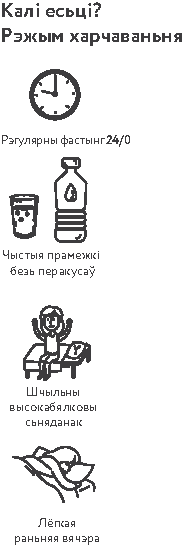
\includegraphics[scale=1.5]{willpower/ch4/2.pdf}
\end{figure}
%((Калі есьці? Рэжым харчаваньня Рэгулярны фастынг 24/0 Сьняданак Абед Вячэра Частыя прамежкі безь перакусаў Аптымальная частасьць харчаваньня Шчыльны высокабялковы сьняданак Звужайце харчовае вакно плыўна 12/12 тыповая 10/14 8/16 папулярная 6/8 4/20 дыета ваяра Лёгкая раньняя вячэра Большую частку калёрыяў зьесьці ўдзень))

\subsection*{Хранабіялёгія харчаваньня}
Акрамя харчовага акна, важна правільна разьмяркоўваць калёрыі на працягу дня. У сучасным сьвеце частым зьяўляецца пропуск сьняданку і багатая вячэра: многія вядуць так званы ``адкладзены'' лад жыцьця, калі людзі імкнуцца ўвечары ``пажыць для сябе'', спажываючы розныя забаўкі і зацягваючы адыход да сну. Пры гэтым менавіта ўвечары людзі больш схільныя да пераяданьня праз стрэс і стому, самакантроль слабее. Якая-небудзь булка ці бігмак смачнейшыя ўвечары, чым раніцай, ці ня праўда?!

Аднак максімальная адчувальнасьць да інсуліну дасягаецца апоўдні, а~мінімальная~--- апоўначы, зьніжаючыся на 54\,\%. Чым больш калёрыяў мы зьядаем позна ўвечары, тым вышэйшыя рызыкі для здароўя і горшыя біямаркеры: расьце ўзровень хранічнага запаленьня, вышэйшая рызыка раку грудзей, павялічваецца нават рызыка атрымаць сонечныя апёкі на наступны дзень!

Наша харчовае вакно і большасьць зьяданых калёрыяў павінны супадаць са сьветлым часам содняў. Яшчэ лепш, калі з~гэтым жа часам супадае і наша працоўная актыўнасьць. Дасьледаваньні паказваюць, што, чым мацнейшае разыходжаньне паміж сьветлавым днём і часам, калі мы ямо, тым шкадней для здароўя. Аптымальна зьядаць раніцай і днём ня менш за 80--85\,\% ад сутачнага каляражу.

\emph{Дыеты, дзе разьмеркаваньне калёрыяў паміж трыма прыёмамі ежы складае 50\,\% на сьняданак, 30\,\% на абед і 20\,\% на вячэру, прыкметна больш карысныя для здароўя, чым з~разьмеркаваньнем 20\,\%, 30\,\% і 50\,\% адпаведна. Такая сыстэма называецца В-дыета (B~--- breakfast) або early Time-Restricted Feeding (eTRF)~--- раньняе кармленьне з~абмежаваньнем па часе, то бок трэба зьядаць сутачны каляраж на працягу першых 8 гадзінаў пасьля абуджэньня. Іншыя сыстэмы рэкамэндуюць яшчэ большы перанос калёрыяў на сьняданак і абед у~суадносінах 7:5:2 (сьняданак, абед і вячэра).}

Дасьледаваньні паказваюць, што людзі, якія рэгулярна сьнедаюць, больш схільныя да зьніжэньня масы цела, чым тыя, хто пэрыядычна прапускае сьняданак . Удзельнікі з~самым вялікім па каляражы сьняданкам дэманструюць больш высокае зьніжэньне вагі, чым удзельнікі з~самым вялікім абедам ці вячэрай.

\subsection*{Колькі разоў на дзень есьці?}
Доўгатэрміновыя дасьледаваньні паказалі, што яда тройчы на дзень дапамагае падтрымліваць нармальную вагу. Таксама для некаторых людзей можа быць карысны рэжым, у~якім ёсьць толькі два прыёмы ежы~--- я прытрымліваюся менавіта такой стратэгіі. Дарэчы, у~некаторых дасьледаваньнях паказана, што дыябэтыкі на двухразовым харчаваньні хутчэй худнеюць і аднаўляюць адчувальнасьць да інсуліну. Дзеці, падлеткі і аслабленыя пасьля захворваньняў людзі могуць есьці часьцей~--- чатыры разы на дзень.

Дробнае харчаваньне нават пры кантролі каляражу ў~доўгатэрміновай пэрспэктыве можа прыводзіць да павелічэньня вагі. Калі ў~дадзены момант вы ясьце шэсьць і больш разоў у~дзень, то зьмяншаць колькасьць прыёмаў ежы трэба плыўна і паступова.

Спажываньне большай часткі каляражу раніцай і днём, абавязковы сьняданак, частата прыёмаў ежы два-тры разы ў~дзень і рэгулярныя пэрыяды фастынгу\index{фастынг}~--- усё гэта вядзе да такіх станоўчых зьменаў, як зьніжэньне хранічнага запаленьня, паляпшэньне цыркаднай рэгуляцыі, павялічаная аўтафагія\index{аўтафагія}, стрэсаўстойлівасьць\index{стрэсаўстойлівасьць} і лепшы стан мікрафлёры.

\subsection*{Сьняданак і вячэра}
Цяпер, калі вы разабраліся з~агульнымі правіламі рэжыму, час перайсьці да прыёмаў ежы: сьняданку, абеду і вячэры. Я рэкамэндую рэгулярна сьнедаць у~адзін і той жа час, на працягу гадзіны-паўтары пасьля абуджэньня~--- не пазьней, і шчыльна, па-каралеўску. Сьняданак павінен складаць ня менш за 30--40\,\% сутачнай калярыйнасьці і зьмяшчаць мінімум 30--40 г бялку. У аснове сьняданку павінны быць якасныя бялковыя прадукты: яйкі, рыба, курыца з~гароднінай і зелянінай, а~ня каша. Да іх можна дадаваць тлушчы і некрухмалістую гародніну. Калі раніцай няма апэтыту, менш ежце на вячэру ці прапусьціце вячэрні прыём ежы.

\begin{figure}[htb]
  \centering
  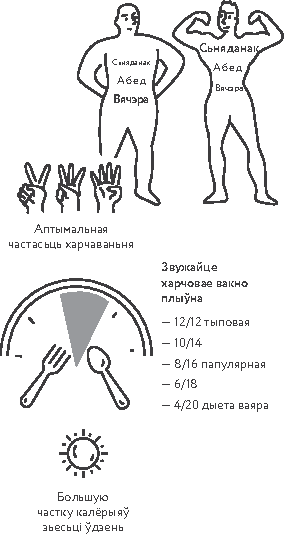
\includegraphics[scale=1.5]{willpower/ch4/3.pdf}
\end{figure}

\emph{Прыклады сьняданкаў, абедаў і вячэр вы можаце знайсьці на маім Youtube-канале, дзе ў~вольным доступе выкладзеныя відэа-ролікі прыгатаваньня страў тыднёвага рацыёну. Заўсёды майце зь вечара плян сьняданку на раніцу, захоўвайце запас замарожанай ежы (агародніна, мяса, рыба, ягады, зеляніна), каб у~выпадку чаго ў~вас быў запасны варыянт сьняданку.}

Шчыльны бялковы сьняданак дапамагае кантраляваць насычэньне, павялічвае ўзровень энэргіі, стабілізуе ваганьні глюкозы ў~крыві. Таксама ён павялічвае стрэсаўстойлівасьць\index{стрэсаўстойлівасьць} і мае шэраг нечаканых эфэктаў, напрыклад павялічвае фертыльнасьць\index{фертыльнасьць}. 

\infobox{Сынхранізуйце свае харчовыя гадзіны, убудаваўшы прыём ежы ў~якасны ранішні рытуал: зарадка, кантрасны ці халодны душ, яркае сьвятло, шчыльны сьняданак, плянаваньне дня і фокус на прыярытэтах.}

Абед павінен быць не занадта позьнім і таксама дастаткова шчыльным прыёмам ежы. А вось вячэраць варта ўмерана: гароднінай і зелянінай з~карыснымі тлушчамі, скажам, аліўкавым. Ня варта ўжываць крупы, гатовыя прадукты і вялікую колькасьць бялку. Аптымальна вячэраць за тры-чатыры гадзіны да сну. Зрэшты, калі вы часам павячэраеце ў~рэстаране позна і з~сацыяльнымі мэтамі, праблемы няма, але не прапускайце на наступны дзень сьняданак. 

\emph{«Пайду праверу, ці выключаны сьвятло на кухні! Вазьмі і мне кавалачак!» Вечар~--- час крушэньня ўсіх надзей на пахуданьне і правільнае харчаваньне. Арганізуйце сабе рытуал на вечар для кантролю пераяданьня: заплянуйце расслабляльныя працэдуры, зрабіце дома няяркае жоўтае сьвятло, каб не зьбіваць ваш унутраны гадзіньнік. Калі ў~вас ёсьць чым заняць сябе, тыя вы ня будзеце шныпарыць па шафках і лядоўні ўвечары. Прадаюцца нават адмысловыя замкі на лядоўню, якія блякуюць доступ да яго ўвечары і ўначы, але я ўпэўнены, што вы дасьце рады і бяз гэтага.}

\subsection*{Харчовы пост ці фастынг\index{фастынг}}
Устрыманьне ад ежы на працягу розных пэрыядаў часу~--- традыцыйная і карысная практыка. Фастынг\index{фастынг}~--- гэта кароткачасовае абмежаваньне паступленьня ежы (калёрыяў), якое практыкуецца сьвядома і рэгулярна для дасягненьня канкрэтнай тэрапеўтычнай мэты.

Фастынг\index{фастынг} валодае мноствам узьдзеяньняў на арганізм чалавека: ад зьніжэньня ўзроўняў ІФР-1 і ўзнаўленьня адчувальнасьці да інсуліну і лептыну, да глыбокіх зьменаў на ўзроўні актыўнасьці генаў. Фастынг паляпшае ліпідны профіль, зьніжае ціск, зьніжае запаленьне, павышае нэўраплястычнасьць\index{нэўраплястычнасьць}, зьніжае акісьляльны стрэс, рызыку анкалягічных, нэўрадэгенэратыўных і сардэчна-сасудзістых захворваньняў\index{сардэчна-сасудзістыя захворваньні}, павышае ўзровень выпрацоўкі гармону росту і адчувальнасьць да інсуліну, нават паляпшае рост карысных бактэрыяў. Фастынг\index{фастынг} вядзе да таго, што арганізм пачынае выпрацоўваць больш кетонавых целаў, і гэта прыводзіць да рэгулярнай актывацыі мэтабалічнага пераключэньня, што карысна для здароўя.

Штодзённы фастынг\index{фастынг}, калі мы скарачаем харчовае вакно, дапамагае на 500 ккал скараціць каляраж і схуднець. Фастынг\index{фастынг} выкарыстоўваецца як для лячэньня захворваньняў, так і для больш спэцыфічных мэтаў~--- паляпшэньне працы мозгу, перазагрузка імуннай сыстэмы\index{імунная сыстэма} і многае іншае. 

\infobox{Галоўнае ў~фастынгу\index{фастынг}~--- гэта рэгулярнасьць і асьцярожнасьць. Калі вы дрэнна пераносіце голад, знаходзіцеся ў~стане стрэсу і нізкай усьвядомленасьці, то фастынг можа вам нашкодзіць.}

Важна не плянаваць галаданьне адразу на некалькі дзён: фастынг\index{фастынг}~--- гэта як шпагат, садзіцца трэба акуратна і павялічваць нагрузку паступова. Ваша стаўленьне да пачуцьця голаду можа або зьніжаць, або павышаць стрэс~--- важна ўспрымаць гэтую практыку як аздараўленьне і дысцыпліну для розуму і цела, а~не як гвалт над сабой.

\subsection*{Варыянты фастынгу\index{фастынг}}
Пропуск прыёмаў ежы. Самае простае, што вы можаце зрабіць,~--- гэта прапусьціць вячэру. Калі ў~вас лёгкі дзень, паездка ці пералёт, то проста не вячэрайце. Пры гэтым шмат піце~--- і больш нічога адмысловага не патрабуецца. Можна так рабіць два-тры разы на тыдзень, празь дзень, прапускаць вячэру~--- гэта просты варыянт фастынгу\index{фастынг}.

\textbf{24/0.} Зручная схэма фастынгу\index{фастынг}, калі вы не ясьце роўна суткі, яна не патрабуе ўваходу і выхаду. Проста сьнедаеце і нічога не ясьце да наступнага сьняданку, п'яце больш воды. Я раблю сутачнае харчовае ўстрыманьне раз на тыдзень~--- у~асноўным з~мэтай большай разумовай яснасьці. А калі вы прапусьціце яшчэ і сьняданак, то атрымаецца каля 36 гадзінаў фастынгу\index{фастынг}. 

Калі вы працуеце, то даўжэйшы пэрыяд галаданьня я не рэкамэндую.

\textbf{36/12, або фастынг\index{фастынг} празь дзень.} Гэта сыстэма, калі вы рэгулярна посьціце 36 гадзінаў, а~ясьце ў~прамежак 12 гадзінаў без абмежаваньняў, пры гэтым колькасьць зьяданых калёрыяў моцна скарачаецца. Гэтая сыстэма мае шмат розных назваў: Alternate-day fasting, Every-Other-Day Diet (EODD), UpDayDownDay. Гэта строгая і складаная сыстэма, але для пэўнага тыпу людзей, якія добра кіруюць пачуцьцём голаду, яна можа падысьці.

\textbf{5:2.} Мяркуе абмежаваньне калярыйнасьці да 500\,ккал у дзень два дні на тыдзень, пры гэтым вы ясьце ў~астатнія дні як звычайна.

\textbf{Дыета, якая імітуе галаданьне (FMD Fasting Mimicking Diet),~---} гэта 5 дзён адмысловай дыеты запар адзін раз на месяц, звычайна пад назіраньнем спэцыялістаў. У першы дзень вы падразаеце свой рацыён напалову, потым ясьце траціну свайго звыклага рацыёну, прыбраўшы жывёльныя бялкі. Рацыён складаецца з~расьлінных бялкоў на 10\,\%, 56\,\% калёрыяў~--- тлушчы, 34\,\%~--- нізкаглікемічныя вугляводы (агародніна, зеляніна і да т.~п.). \textbf{Аўтары гэтай дыеты рэкамэндуюць здаровым людзям праходзіць адзін такі цыкл раз на тры месяцы.}

\textbf{Працяглыя сыстэмы галаданьня.} На маю думку, любыя сыстэмы фастынгу\index{фастынг} працягласьцю больш за тры дні павінны праходзіць пад кантролем спэцыялістаў, інакш рызыка пабочных эфэктаў можа перавысіць карысьць. 

\emph{Папулярны лёзунг ``больш трэніруйся, меней еж'' прыводзіць да шматлікіх ускладненьняў: парушэньня харчовых паводзінаў, скокаў вагі, парушэньня цыклю і да т.~п. У жанчынаў праз пастаяннае недаяданьне можа разьвіцца так званая ``спартыўная жаночая трыяда'', якая ўключае адмыслова зроблены дэфіцыт калёрыяў, парушэньне цыклю і астэапароз. Ня варта ствараць дэфіцыт калёрыяў больш за 10\,\%, практыкаваць ``паскоранае пахуданьне''~--- гэта шкодна і небясьпечна.}

\textbf{Чым жа фастынг\index{фастынг} лепшы за звычайнае штодзённае абмежаваньне калёрыяў?} Клясычнае абмежаваньне калёрыяў мае насамрэч шмат мінусаў: псыхалягічна цяжка ў~доўгатэрміновай пэрспэктыве дакладна лічыць калёрыі, ёсьць праблемы і з~арганізмам~--- ад стану костак да аслабленьня імунітэту. Фастынг\index{фастынг} просты, бо лічыць колькасьць гадзінаў прасьцей, чым калёрыяў. Пры гэтым адсутнічае пастаяннае харчовае абмежаваньне, дапушчальныя варыяцыі па ежы, дасягаецца выдатны кантроль голаду і апэтыту.

Дасьледаваньні, якія параўноўваюць хранічнае абмежаваньне калёрыяў з~фастынгам\index{фастынг} празь дзень, паказалі, што па большасьці паказьнікаў нават на прамежку 12 месяцаў паміж імі няма адрозьненьняў. Іншыя дасьледаваньні паказваюць на эфэктыўнасьць фастынгу\index{фастынг} празь дзень у~дачыненьні да большага скіду вагі і больш выяўленага паляпшэньня шэрагу паказьнікаў, напрыклад адчувальнасьці да інсуліну.

\emph{Фастынг\index{фастынг} можа быць проціпаказаны людзям з~захворваньнямі страўнікава-кішачнага тракту, з~гісторыяй парушэньняў харчовых паводзінаў, парушэньнямі мэнструальнага цыклю і да т.~п. Для бясьпекі фастынгу\index{фастынг} важна пазьбягаць абязводжваньня і быць занятым. У цэлым жанчынам рэкамэндуюцца больш ашчадныя сыстэмы фастынгу\index{фастынг}, чым мужчынам. Так, ім часьцей камфортнейшыя 3, а~не 2 прыёмы ежы, 10/14, а~не 8/16 у~параўнаньні з~мужчынамі.}

Каб узмацніць эфэкт фастынгу\index{фастынг} і яго пераноснасьць, важна дадаць больш умеранай актыўнасьці ў~выглядзе хады, велашпацыраў, бегу трушком. У доўгатэрміновай пэрспэктыве важна ацэньваць пераноснасьць і эфэктыўнасьць фастынгу\index{фастынг}, ацэньваючы ўзровень палавых гармонаў, С-рэактыўнага бялку, адчувальнасьці да інсуліну. Можна выкарыстоўваць вымярэньне ўзроўню кетонавых целаў у~праграме фастынг-трэкеру ў~тэлефоне для аптымізацыі працэсу.

\subsection*{Пытаньні і заданьні}

1. Пачніце нармалізацыю харчаваньня з~усталяваньня рэгулярнага рэжыму і захаваньня чыстых прамежкаў.

2. Рэгулярна сьнедайце і абедайце, паспрабуйце часам прапусьціць вячэру, звузіўшы сваё харчовае вакно.

3. Абярыце самы спакойны дзень і зрабіце 24-гадзіннае харчовае ўстрыманьне, калі ў~вас няма да гэтага мэдыцынскіх проціпаказаньняў.


\section{Арганізацыя трапезы. Як есьці?}

Фаіна Ранеўская неяк сказала: «Даражэнькая, калі хочаце схуднець~--- ежце голай і перад люстэркам». Магчыма, гэта спрацуе, але ёсьць і менш экстравагантныя спосабы арганізаваць працэс ежы так, каб зьесьці меней і з~большым задавальненьнем. На жаль, сёньня людзі ядуць вельмі хутка, адцягваючыся на смартфоны і сэрыялы і не надаючы належнай увагі ежы. Гэта вядзе да аўтаматычнага пераяданьня.

Калі вы добра ясьце, то і больш насалоджваецеся смакам, колерам і пахамі, становіцеся больш сытымі і здаволенымі~--- а~значыць, будзеце зь лёгкасьцю прытрымлівацца такой сыстэмы харчаваньня. Важна падтрымліваць пастаянны рэжым харчаваньня бяз рэзкіх зьменаў часу сьняданку, абеду і вячэры: тады арганізм наладжвае ўнутраны гадзіньнік і пачынае рыхтавацца да сталаваньня загадзя. 

\infobox{Пры арганізацыі яды важна ўсё: час прыёму ежы, выбар прадуктаў, атрыманьне задавальненьня, папярэдні апэтыт і пачуцьцё насычэньня пасьля яды.}

Для таго каб прытрымлівацца свайго харчаваньня ў~доўгатэрміновай пэрспэктыве, трэба кантраляваць голад і сытасьць. Калі вас мучыць голад днём ці ўвечары або вы ясьце зусім без апэтыту, то ня зможаце доўга пратрымацца ў~гэтым рэжыме на адной сіле волі. Таму важна пачаць назіраць за сваім голадам і сытасьцю, вывучаць, што і як на іх уплывае.

\begin{figure*}[tb!]
  \centering
  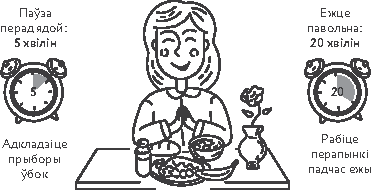
\includegraphics[scale=1.5]{willpower/ch4/4.pdf}
\end{figure*}

\textbf{Схэму харчаваньня плянуйце ад сьняданку:}
\begin{itemize}
  \item шчыльны сьняданак, каб насычэньня хапіла да абеду;
  \item абед, каб насычэньня хапіла да вячэры;
  \item вячэра, каб насычэньня хапіла да сну, але і лёгкая пры гэтым, каб раніцай быў апэтыт.
\end{itemize}

Невыпадкова ў~народзе кажуць, што ``апэтыт прыходзіць падчас яды'', бо ўзровень ``гармону голаду'' грэліну расьце, калі мы проста глядзім на ежу. 

\textbf{Чым даўжэй глядзім, атрымліваем асалоду ад водару і прыгожага выгляды, тым вышэйшы ўзровень грэліну і лепшы апэтыт.} Фон апэтыту важны для распазнаньня сапраўднага насычэньня: калі вы пачынаеце есьці, высокі ўзровень грэліну падае, і арганізм такім чынам атрымлівае сыгнал аб сытасьці. Калі вы пачалі есьці зь нізкім грэлінам, гэта значыць без апэтыту, то вы лёгка пераядаеце!

Добра адрэгуляванае пачуцьцё голаду падказвае важнае правіла: ежце, калі адчуваеце фізычны голад, і ежце да пачуцьця насычэньня. Фізычны голад~--- гэта проста сыгнал арганізма, як чырвоная лямпачка на бензабаку, што запас глікагену ў~печані памяншаецца і трэба яго папоўніць. Дарэчы, гармон грэлін станоўча ўзьдзейнічае на здароўе: умацоўвае імунітэт, павялічвае ўзровень дафаміну, умацоўвае і амалоджвае цягліцы. 

\textbf{Успрымайце лёгкае пачуцьцё голаду станоўчаа, бо гэта смак да жыцьця, ён ``уключае'' рэжым паляўнічага і пошуку ежы.}

\textbf{Вызначайце эмоцыі, вырашайце рэальныя праблемы, не заядайце~--- і паступова вы будзеце ўсё лепш адрозьніваць фізычны голад і эмацыйны.} Важна навучыцца адрозьніваць фізычны голад ад эмацыйнага, які можа ўзьнікаць у~адказ на стрэс, нэгатыўныя эмоцыі, стомленасьць. Але эклер ці піца не дапамогуць вырашыць вашыя працоўныя праблемы. Каб навучыцца выразна адрозьніваць іх, памятайце, што фізычны голад узьнікае паступова, можа быць адкладзены, пры ім вы гатовыя есьці што заўгодна. А вось эмацыйны голад часта ўзьнікае раптоўна, бяз сувязі з~папярэдняй ежай, пры ім хочацца зьесьці крыху, але пэўных прадуктаў~--- салёнага, хрумсткага, салодкага, тлустага, вэнджанага, а~яшчэ лепш~--- усё гэта разам. Бо яшчэ тысячы гадоў таму людзі заўважылі: «Лепей міска гародніны і зь ёю любоў, чым укормлены бык і зь ім нянавісьць» (Выслоўі 15:17).

\textbf{Рэарганізуйце час прыёму ежы:}
\begin{enumerate}
  \item Зрабіце паўзу перад ядой.
  \item Ежце павольна~--- аптымальны час складае 15--20 хвілін.
  \item У час яды рабіце перапынкі на пару хвілінаў~--- адчуйце, ці сапраўды вы хочаце працягнуць прыём ежы.
  \item Ежце сьвядома і атрымлівайце больш некалярыйнага задавальненьня.
  \item Калі паелі~--- ``завяршыце сталаваньне''.
\end{enumerate}

\subsection*{А зараз падрабязьней}
Правіла паўзы перад ядой. Сядзьце за стол і не пачынайце адразу есьці, пачакайце 1--3 хвіліны. Паглядзіце на стравы, панюхайце, расслабцеся. Падумайце пра ежу як крыніцу энэргіі, якая патрэбная вам для вырашэньня важных справаў. Цікава, што ў~першыя сэкунды зьяўляецца жаданьне зьесьці болей, але дзьве і больш хвіліны нюху зьмяншаюць цягу і дапамагаюць абраць больш здаровыя стравы. Выпіце шклянку вады~--- гэта дапаможа зьесьці менш. 

Таксама карысна ўспомніць, што вы елі ў~мінулы прыём ежы, і сфатаграфаваць ежу ў~выгадным ракурсе~--- гэта дапаможа атрымаць больш задавальненьня і насыціцца меншай колькасьцю ежы. Выкладваць кожны раз фота ў~інстаграм зусім не абавязкова.

\infobox{Падумайце пра харошае, няхай у~роце зьявіцца сьліна~--- гэта значыць, што актыўнасьць стрэсавай сымпатыйнай сыстэмы зьніжаецца, і вы гатовыя да прыёму ежы. Заўсёды памятайце, што ежа~--- гэта сапраўдны дар, які мы прымаем зь любоўю і падзякай, які дае нам сілы жыць і радавацца жыцьцю.}

\subsection*{Правіла павольнай яды}
Калі я працаваў анэстэзіёлягам-рэ\-ані\-ма\-то\-ля\-гам, важным навыкам было паесьці вельмі хутка. Гэта ўвайшло ў~звычку, мне складана было потым перавучыцца і пачаць есьці павольна. Затое цяпер павольная дыета~--- slow food~--- мабыць, адзіная з~усіх дыетаў, якую я магу рэкамэндаваць кожнаму без асьцярогаў.

\emph{Устаноўлена, што хуткая ежа зьвязаная з~рызыкай пераяданьня, атлусьценьня\index{атлусьценьне} і дыябэту\index{дыябэт}. Павольная ежа дазваляе зьесьці менш і пры гэтым адчуваць сябе больш сытым. Паглядзіце па сэкундамэры, зь якой хуткасьцю вы ясьце і ці трэба вам запавольвацца.}

Для таго каб есьці павольна, важна старанна жаваць, ня есьці адначасова са смартфонам, карыстацца прыборамі, адразаць невялікія кавалачкі. Ужывайце менш здробненай ежы: выбірайце мяса замест катлетаў, цэльную садавіну, а~ня смузі. Недастатковае перажоўваньне часта спадарожнічае хуткай ежы.

Пэрыядычна варта рабіць \textbf{чыстыя паўзы}, калі ў~роце ўжо нічога няма, але прыборы вы адклалі ўбок. У гэтыя перапынкі паміж ядойй можна пагутарыць з~тымі, з~кім вы падзяляеце стол.

Прыём ежы важна \textbf{правільна завяршыць}, каб вы былі ўпэўнена сытыя і задаволеныя. Падумайце, што вы яшчэ хочаце зьесьці ці выпіць? Невялікі смачны дэсерт у~выглядзе арэхаў ці садавіны, ягадаў, горкай чакаляды дапаможа вам атрымаць яшчэ большае задавальненьне ад сталаваньня. Пасьля прапалашчыце рот, але ня чысьціце зубы, асабліва калі елі садавіну.

\subsection*{Атрымлівайце задавальненьне ад ежы}
Задавальненьне ад ежы ўплывае на пачуцьцё сытасьці. Мы можам павялічыць задавальненьне калярыйным і некалярыйным спосабамі~--- перавагу аддаём, вядома, апошняму. Чым прыгажэй будзе сэрвіраваны ваш стол, тым смачнейшай будзе ежа. Прыгожа раскладзіце ежу ў~прыгожыя талеркі, выкарыстоўвайце прыборы, а~ўвечары запаліце сьвечку. Успомніце, наколькі смачнейшай здаецца звычайная ежа ў~раскошным рэстаране ці на пікніку на беразе мора. \textbf{Любімыя смакі, сэрвіроўка, кампанія, месца прыёму ежы~--- усё гэта мае значэньне і абмяжоўваецца толькі вашай фантазіяй.}

\subsection*{Арганізуйце рытуал прыёму ежы}
Памятаеце сабак Паўлава? Вялікі навукоўца выявіў рэфлексы на прыкладзе выдзяленьня страўнікавага соку ў~сабак у~адказ на розныя стымулы, у~тым ліку і нехарчовыя, напрыклад гук званочка. Вы можаце выпрацаваць у~сябе такія ж рэфлексы, засьцілаючы стол абрусам перад ежай і прыбіраючы яго пасьля. \textbf{З гэтай жа прычыны важна есьці толькі на кухні ці ў~гасьцёўні, а~не на працоўным месцы ці ў~ложку, інакш там будзе ўвесь час зьяўляцца апэтыт.}

\textbf{Усьвядомленае харчаваньне~---} эфэктыўны спосаб есьці менш і быць больш сытымі. Успомніце, які кавалачак марожанага самы смачны? Першы і апошні! А чаму? Бо мы зьвяртаем на іх больш увагі. Калі вы трымаеце ўвагу на ежы, на тым, як зьмяняецца яе смак і кансыстэнцыя, то задавальненьня больш. Будзьце ўсьвядомленыя і сканцэнтраваныя на ежы, гэта складана, але паступова трэніруецца. Паўтаруся: ежа з~праглядам тэлевізара, гартаньнем стужкі смартфона або чытаньнем кнігі зьвязаная зь большым пераяданьнем і меншым задавальненьнем.

\infobox{Сытасьць цікавым чынам зьвязаная з~павагай да ежы. Людзі, якія лічаць сваю порцыю больш сытнай, паказваюць значнае зьніжэньне гармону голаду грэліну. Нядзіўна, што і кошт віна ўплывае на яго смак.}

\begin{figure}[ht!]
  \centering
  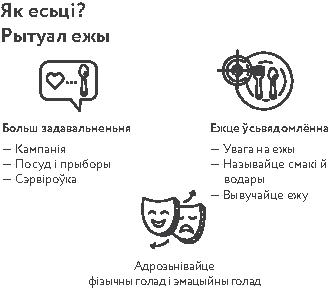
\includegraphics[scale=1.3]{willpower/ch4/5.pdf}
\end{figure}

Адным з~выдатных інструмэнтаў павышэньня некалярыйнага задавальненьня зьяўляецца разьвіцьцё смаку. Чым больш характарыстык ежы мы можам назваць, тым больш атрымліваем уражаньняў і стымулаў. Для гэтага трэба пашыраць свой слоўнікавы запас, апісваць смак, выгляд, пах кожнага прадукту, даваць адценьні базавым смакам: салодкае, салёнае, кіслае, горкае, умамі,~--- і іх узаемадзеяньню паміж сабой. Рабіцеся гурманамі!

\subsection*{Пазбаўцеся ад стымулятараў апэтыту}
Сярод прадуктаў і дадаткаў ёсьць тыя, якія насычаюць, і тыя, якія ўзмацняюць апэтыт. Стымулююць пераяданьне смажанае ці вэнджанае, соль, цукар, араматызатары, фарбавальнікі, цукразаменьнікі, узмацняльнікі смаку, а~таксама іх спалучэньні. Насычаюць~--- клятчатка, зеляніна, спэцыі, гарэхі. Зьніжаюць апэтыт горкі і кіслы смакі. Сярод нутрыентаў добра насычае бялок, ён дае доўгую сытасьць. Невялікія колькасьці тлушчу запавольваюць пэрыстальтыку і могуць падоўжыць пачуцьцё сытасьці.

\emph{Важным кампанэнтам сытасьці з'яўляецца аб'ём зьедзенага: калі павялічыць колькасьць прадуктаў зь нізкай удзельнай шчыльнасьцю, вы зможаце есьці болей аб'ёму і меней калёрыяў. Напрыклад, у~кашу варта дадаць болей гародніны і зеляніны.}

\begin{figure*}[tb!]
  \centering
  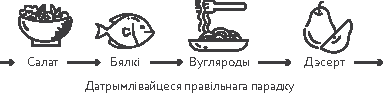
\includegraphics[scale=1.5]{willpower/ch4/6.pdf}
\end{figure*}

\subsection*{Цьвёрдая дыета}
Цяпер модна многія прадукты ёсьць у~здробненым выглядзе: супы-пюрэ, катлеты, фрэшы. Жаваньне вельмі важнае ня толькі для насычэньня, але і для мозгу~--- гэты працэс павышае сытасьць і зьніжае ўзровень гармону стрэсу картызолу. У жывёльных мадэлях навукоўцы выявілі, што мяккая здробненая ежа (soft diet) прыводзіла да зьніжэньня працоўнай памяці, зьніжэньня нэўрагенэзу ў~гіпакампе, павелічэньня рызыкі нэўрадэгенэратыўных захворваньняў. Таму карысна пагрызьці гародніну і пажаваць мяса~--- як для дзяцей, каб правільна фармаваўся тварны шкілет, так і для дарослых, каб адчуваць сябе больш сытымі. \textbf{Грызіце гародніну, а~не сябе ці навакольных!}

\subsection*{Датрымлівайцеся правільнага парадку страваў}
Старажытныя рымляне, якія любілі парадак, складалі сваё сталаваньне па пляне ``ab ovo usque ad mala'', то бок пачыналі зь яек, а~заканчвалі яблыкамі (садавіной). Сучасныя дасьледаваньні пацьвярджаюць традыцыйную эмпірычную ідэю аб тым, што парадак страваў важны для здароўя: пры аднолькавым складзе і каляражы гэты парадак істотна ўплывае на нашыя гармоны.

\emph{Некаторыя прадукты могуць уплываць на выпрацоўку гармону GLP-1, які запавольвае апаражненьне страўніка і падаўжае насычэньне. Ніжэйшая хуткасьць апаражненьня страўніка зьвязаная зь лепшым насычэньнем і павольнейшым паступленьнем ежы ў~тонкі кішачнік, павольнейшым яе ўсмоктваньнем. А чым павольней, тым меншая постпрандыяльная глікемія~--- залішні ўздым глюкозы ў~крыві пасьля яды. Такая глікемія зьяўляецца раньняй прыкметай дыябэту\index{дыябэт}, а~таксама можа ўзьнікаць і ў~(пакуль) здаровых людзей, узмацняючы выяўленасьць глікацыі, аксідантнага стрэсу і падвышаючы рызыку сардэчна-сасудзістых хваробаў.}

Калі вы ясьце гародніну перад прыёмам вугляводаў больш высокай калярыйнай шчыльнасьці і больш высокага глікемічнага індэксу, гэта паляпшае глікемічны кантроль: меней інсуліну, меншы ўздым глюкозы. Калі вы зьядаеце першым бялок, то гэта таксама паляпшае глікемічны кантроль. Пачынайце сталаваньне зь бялковых прадуктаў, гародніны, багатых клятчаткай, і тлушчаў: напрыклад, спачатку салата з~аліўкавым алеем, затым бялковы прадукт і толькі пасьля гэтага вугляводны гарнір ці садавіна.

\subsection*{Пытаньні і заданьні}

1. Ежце заўсёды ў~адным месцы, без тэлефона ў~руках.

2. Уключайце сэкундамэр і павялічвайце час ежы.

3. Купіце сабе прыгожыя талеркі і прыборы.


\section{Прадукты: агульныя крытэры выбару. Што есьці?}

У гэтай главе сфармулюем агульныя правілы, якія дапамогуць вам рабіць самы здаровы выбар у~любой прадуктовай групе. Сярод правілаў харчаваньня ёсьць шэраг унівэрсальных, якія пасавацьмуць любому чалавеку зь любым стылем харчаваньня. Яны простыя, але пры гэтым навукова абгрунтаваныя і эфэктыўныя. Паспрабуйце іх прытрымлівацца, і вы ў~дастаткова хуткім часе зможаце ўбачыць вынікі.

\textbf{Агульныя крытэры выбару ўключаюць:}
\begin{itemize}
  \item выбар цэльных прадуктаў;
  \item выбар прадуктаў зь нізкай калярыйнай і высокай біялягічнай шчыльнасьцю;
  \item выбар сьвежых прадуктаў;
  \item выбар прадуктаў з~ашчаднай апрацоўкай;
  \item разнастайны прадуктовы кошык.
\end{itemize}

Усё, што мы ямо, можна ўмоўна падзяліць на дзьве групы.

Першая~--- гэта цэльныя прадукты, якія вырасьлі самі: яблык, яйка, рыба, арэх.

Другая~--- харчовыя рэчывы, зробленыя зь перапрацаваных субстанцый: мука, дрожджы, соль, цукар, крухмал, сухое малако, сурымі, сухі яечны парашок, соевы парашок, алеі, транстлушчы, разнастайныя харчовыя дабаўкі і да т.~п. Камбінацыі гэтых рэчываў ствараюць штучныя (ультрапэрапрацаваныя) прадукты харчаваньня.

Апрацоўка ўключае ўсе віды ўзьдзеяньня: драбненьне, тэрмаапрацоўку, кансэрвацыю, рафінаваньне, уключэньне ў~склад іншых харчовых субстанцый для зьмены смаку, ачыстку, дэзадараваньне, адбелку і да т.~п. Калі для жывёлаў нават адно здрабніць ежу, то ў~параўнаньні з~кантрольнай групай яны зьядаюць яе на 30\,\% і набіраюць вагу. Чым глыбейшая апрацоўка прадукту, тым больш у~прадукце калёрыяў і харчовых дабавак, тым менш карысных кампанэнтаў і горшае яго засваеньне. Напрыклад, цэльны авёс мае глікемічны індэкс 40, а~аўсяная каша хуткай гатоўкі~--- 80.

\emph{Паляўнічыя-зьбіральнікі выкарыстоўваюць цэльныя прадукты зь мінімальнай апрацоўкай, смажаньнем і варкай. І нават калі ў~іх ёсьць лішак прадуктаў, яны не пераядаюць.}

Памідор~--- гэта не тое ж самае, што кетчуп з~даданьнем солі і цукру, а~цэльнае мяса адрозьніваецца ад смажаных сасісак; сок шкодны, у~адрозьненьне ад цэльнага фрукта. Аддаючы перавагу цэльным прадуктам, мы можам прыкметна зьнізіць рызыкі для здароўя і атрымаць шмат плюсаў. Старайцеся ня менш за 80\,\% свайго рацыёну складаць з~цэльных прадуктаў.

\emph{Ясная рэч, ідэальныя прадукты нам не заўсёды даступныя. Але рыба глыбокай замарозкі супастаўная з~астуджанай па карысных якасьцях, а~вось яе розьніца з~замарожанымі рыбнымі катлетамі ці крабавымі палачкамі будзе вялікая.}

Глыбокая апрацоўка вядзе да страты карысных спалучэньняў, пагаршэньня якасьці прадукту, уключэньня ў~яго вялікай колькасьці дабавак, такіх як схаваны цукар і соль. Перапрацаваная ежа можа нават цалкам супадаць па калярыйнасьці і макронутрыентах, але пры гэтым інакш узьдзейнічаць на харчовыя паводзіны чалавека.

\begin{figure}[ht!]
  \centering
  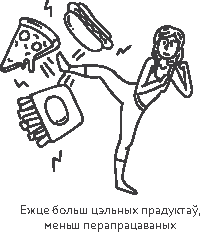
\includegraphics[scale=1.5]{willpower/ch4/7.pdf}
\end{figure}

\infobox{Дасьледаваньні паказалі, што прадукты з~высокай ступеньню апрацоўкі горш насычаюць, зьядаюцца на 50\,\% хутчэй і людзі зьядаюць да дасягненьня сытасьці цэльных прадуктаў на 2500 супраць 3000\,ккал перапрацаваных. }

Гэта значыць проста пераход на цэльныя прадукты можа скараціць пераяданьне на 500\,ккал у~дзень~--- без пачуцьця голаду! Іншыя дасьледаваньні пацьвярджаюць, што перапрацаваныя прадукты правакуюць набор вагі, павялічваюць рызыку сардэчна-сасудзістых захворваньняў\index{сардэчна-сасудзістыя захворваньні} і зьніжаюць працягласьць жыцьця. Кожныя 10\,\% калёрыяў з~ультрапэрапрацаваных прадуктаў на 10\,\% павялічваюць рызыку разьвіцьця раку. Даданьне цукру, солі, тлушчу ў~прадукты ўзмацняе цягу да іх, іх эфэкт падсумоўваецца.

Часта людзі, якія хочуць палепшыць сваё харчаваньне, трапляюць у~пастку псэўдакарысных прадуктаў. Псэўдакарысныя прадукты~--- гэта перапрацаваныя прадукты, якія выдаюць сябе за здаровыя, але такімі не зьяўляюцца. Да іх адносяцца сокі, сухафрукты, цукразаменьнікі, розныя віды ``карыснай'' мукі, ``карысныя прысмакі'', расьліннае малако, вэганскія соевыя сасіскі ды іншае, што прысутнічае ў~выглядзе слоікаў, пакетаў, бутэлек, а~ня цэльных прадуктаў. Для іх продажу выкарыстоўваюцца розныя маркетынгавыя прыёмы, ствараецца арэол здаровага харчаваньня, калі даданьне аднаго карыснага кампанэнта мяняе наша ўспрыманьне прадукту.

\emph{Напрыклад, печыва зь вітамінамі здаецца нам больш здаровым. Але зь печывам нічога не адбылося, яно засталося ранейшымі. Або адзін маленькі ліст салаты ў~гамбургеры зьмяншае яго ўспрыманую каларыйнасьць, пасыпка семкамі робіць батон больш ``здаровым''. Часта выкарыстоўваецца акцэнт на адным кампанэнце, напрыклад упор на карысьць пэктыну ў~зэфіры. Але зэфір~--- гэта перадусім цукар, а~пэктын мы атрымліваем, зьеўшы звычайны яблык. Карысныя прысмакі часта ўяўляюць сабой проста іншыя формы цукру. Усе цукры біяэквівалентныя: цукар зь мёду ці фінікаў сапраўды гэтак жа ўплывае на наша здароўе, як і звычайны белы цукар. Надпісы ``эка'', ``бія'', ``фрэш'', ``raw'', ``вэган'', ``фэрмэрскі'', ``арганічны'', ``нізкакалярыйны'', ``здаровы'', ``без даданьня цукру'' і да т.~п. могуць прысыпаць нашу пільнасьць.}

\subsection*{Правіла калярыйнае шчыльнасьці}
Старайцеся выбіраць ежу зь сярэдняй і нізкай удзельнай калярыйнай шчыльнасьцю, то бок невысокай колькасьцю калёрыяў у~адзінцы аб'ёму. Крупы, батончыкі, гатовая ежа ўтрымліваюць шмат калёрыяў у~малым аб'ёме, і іх пераесьці. Акрамя гэтага, канцэнтраваныя прадукты аказваюць нэгатыўнае ўзьдзеяньне на мікрафлёру, выклікаючы запаленчы адказ. Звычайна ў~прадуктах зь нізкай удзельнай каларыйнасьцю больш карысных кампанэнтаў, якія ўключаюць клятчатку, вітаміны, мінэралы і да т.~п.

\emph{Напрыклад, мы можам выбіраць ня хлеб, белы рыс ці пасту, а~моркву ці гарбуз. Гэтае правіла тычыцца ня толькі вугляводаў: напрыклад, марская рыба мае ўдзельную калярыйнасьць амаль у~два разы меншую, чым сьвініна.}

\textbf{Зьменшыце долю прадуктаў з~высокай калярыйнай шчыльнасьцю,} г.~зн. «бедных прадуктаў», у~якіх шмат калёрыяў і мала нутрыентаў. У першую чаргу гэта тычыцца мучных і кандытарскіх вырабаў, якія зьмяшчаюць шмат цукру і тлушчу. Нават проста крупы, якія зьядаюцца асобна, ня будуць здаровым выбарам: абавязкова дадавайце ў~кожны прыём ежы больш зеляніны і гародніны, каб калярыйныя прадукты займалі меншую частку талеркі.

\textbf{Павялічце частку прадуктаў з~высокай біялягічнай каштоўнасьцю,} г.~зн. «багатых прадуктаў», якія ўтрымліўваюць мала калёрыяў, але шмат карысных злучэньняў, уключаючы фітанутрыенты, клятчатку~--- гэта ліставая зеляніна, ягады, водарасьці, грыбы, гарэхі, насеньне, парасткі і да т.~п. Нават невялікая порцыя гарэхаў робіць прыкметнае дадатнае ўзьдзеяньне на арганізм, зьмяншаючы рызыкі захворваньняў, паляпшаючы абмен халестэрыну. Зеляніна, грыбы і водарасьці можна сьмела патроху дадаваць амаль да любой стравы. Калі зімой зеляніна і ягады недаступныя, выкарыстоўвайце замарожаную зеляніну або высушаныя водарасьці, пасыпайце ежу сушанымі травамі ды спэцыямі. Гэта міт, што спэцыі правакуюць язву страўніка і ўзмацняюць апэтыт: наадварот~--- зьніжаюць колькасьць зьедзенага, станоўча ўплываюць на здароўе. Важна толькі выкарыстоўваць цэльныя спэцыі, а~ня сумесі з~сольлю, глутаматам і ўзмацняльнікамі смаку.

\begin{figure}[ht!]
  \centering
  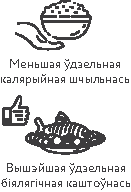
\includegraphics[scale=1.5]{willpower/ch4/8.pdf}\quad
  
\includegraphics[scale=1.5]{willpower/ch4/9.pdf}
\end{figure}

\subsection*{Правіла разнастайнага харчаваньня}
Важна не замыкацца на невялікай колькасьці прадуктаў: чым разнастайней мы ямо, тым лепей закрываем свае запатрабаваньні ў~неабходных арганізму спалучэньнях. Добра, калі ў~нас за сталом на працягу дня розныя прадуктовыя групы, стравы не паўтараюцца, а~за прыём ежы мы зьядаем ня менш за 5--7 розных прадуктаў.

У тыповым рацыёне сучаснага чалавека вельмі часта адсутнічаюць цэлыя групы прадуктаў. На гэта ўплываюць розныя модныя тэндэнцыі, ненавуковыя тэсты на ``непераноснасьць'', дэманізацыя тых ці іншых прадуктаў. Заўсёды імкніцеся пакаштаваць што-небудзь новае, каб узбагаціць свой рацыён. Сярод лінейкі падобных прадуктаў вы можаце выбраць тыя, якія вамі лепш пераносяцца ці здаюцца смачнейшымі: не ідзе фасоля~--- паспрабуйце нут або сачавіцу, не смакуе цыбуля~--- пакаштуйце кінзу, не падабаецца вішня~--- ежце больш чарніц.

Разнастайнасьць дыеты~--- гэта добра, але разнастайнасьць на стале падчас прыёму ежы правакуе пераяданьне. Таму карысна абмежаваць колькасьць прадуктаў, гэта зьмяншае цягу. Калі харчовая ўзнагарода невялікая (простая ежа) і аднастайная (рыба і гародніна, а~ня поўны швэдзкі стол), то людзі ядуць менш. Посьпех монадыетаў і спалучаны з~тым, што такая аднастайная ежа зьніжае да яе цікавасьць. Сёньня ж разнастайнасьць прадуктаў зашкальвае, і ў~краме можна знайсьці дзясяткі тысячаў відаў прадуктаў харчаваньня. 

\infobox{Ежце простую ежу, розныя прадукты ў~розныя прыёмы ежы і мінімум розных прадуктаў у~адзін прыём ежы! Ідэальнага прадукту, які зьмяшчае ў~сабе ўсё неабходнае, не існуе.}

\subsection*{Правіла ашчаднай апрацоўкі}
Пры тэрмаапрацоўцы многіх прадуктаў могуць утварацца канчатковыя прадукты глікацыі~--- іх называюць КПГ або Age, мы іх бачым як брунатна-карычневае адценьне або скарыначку. Запяканьне, вэнджаньне, смажка максімальна павялічваюць утрыманьне КПГ. \textbf{Пры гэтым смажанае здаецца нам смачнейшым~--- такая эвалюцыйная спадчына чалавека.}

Фастфуд\index{фастфуд} зьмяшчае шмат КПГ: смажанае мяса, бэкон, выпечка, бульба і да т.~п. Асабліва інтэнсіўна КПГ утворыцца, калі пры высокіх тэмпэратурах спалучаюцца бялок і цукар. Чым большы кантакт з~паветрам, чым вышэйшая тэмпэратура, чым большы час гатаваньня, тым большы КПГ. 

\infobox{Лішак КПГ павялічвае ўзровень акісьляльнага стрэсу, хранічнага запаленьня, зьніжае адчувальнасьць да інсуліну.}

Самыя ашчадныя спосабы гатаваньня~--- варэньне і гатаваньне на пары. Мяса можна марынаваць у~кіслых субстанцыях (воцат, цытрына) з~дадаткамі, якія зьніжаюць утварэньне КПГ, -- напрыклад, з~размарынам. Ашчаднае гатаваньне таксама дапамагае зрабіць гародніну больш карыснай, паніжаючы яе глікемічны індэкс. Гародніну важна варыць не да мяккага стану, пакідаць яе цьвёрдай. Карысна дадаваць больш сырой неапрацаванай ежы ў~выглядзе зеляніны і гародніны, яна валодае мінімальнай глікемічнай нагрузкай. Цікава, што сырая і вараная гародніна па-рознаму ўплываюць на мікрафлёру. Заліваць крупы вадой можна ня толькі для зьніжэньня ўтрыманьня ў~іх фітатаў, але й для хутчэйшага гатаваньня: вы можаце не варыць аўсянку, а~заліць яе кіпнем, а~грэчку можна на ноч заліць кефірам.

\subsection*{Пытаньні і заданьні}

1. Трымайце дома запас цэльных прадуктаў, навучыцеся іх гатаваць.

2. Ежце больш па аб'ёме, але менш па калёрыях.

3. Бярыце на спробу новыя прадукты ў~краме, каштуйце новае ў~падарожжах.


\section{Вугляводы}

Вугляводы часта абвінавачваюць ва ўсіх грахах. Сапраўды, ня ўсе вугляводы аднолькава карысныя, бо яны ўяўляюць сабой вельмі разнастайную групу прадуктаў харчаваньня.

\textbf{Упарадкуйце свае вугляводы:}
\begin{itemize}
  \item прыбярыце крыніцы даданага цукру;
  \item зьменшыце глікемічную нагрузку: больш зеляніны і гародніны, менш крупаў і мучнога;
  \item павялічце колькасьць харчовых групаў розных расьлінаў: гародніна, зеляніна, садавіна, ягады;
  \item ежце якасныя расьлінныя прадукты зь мінімальнай апрацоўкай, яны павінны складаць аснову здаровага рацыёну.
\end{itemize}

\begin{figure*}[tb!]
  \centering
  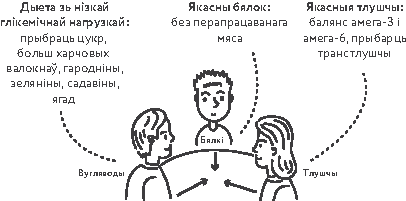
\includegraphics[scale=1.5]{willpower/ch4/10.pdf}
\end{figure*}

\emph{Plant based diet~--- так званая дыета, заснаваная на расьлінах,~--- прапануе зьядаць ня менш за 500 г зеляніны, гародніны і садавіны ў~дзень, а~калі больш, то яшчэ лепш.}

\subsection*{Мінімізуйце даданы цукар} 
Нормай даданага цукру зьяўляецца ня больш за 5\,\% агульнага каляражу. Важна максімальна скараціць яго колькасьць. Зьвярніце ўвагу, што ўсе віды цукру біяэквівалентныя, то бок мёд, кляновы сіроп ці сок белага вінаграду дзейнічаюць аднолькава, таксама як і агава, фінікавы цукар, цукровы трыснёг, какосавы цукар, глюкоза-фруктозны сіроп і яшчэ дзясятак назваў. Цукар ёсьць ня толькі ў~салодкім, яго шмат у~хлебе, соўсах, паўфабрыкатах. Скараціўшы колькасьць цукру, вы зьнізіце і колькасьць зьяданай ежы, бо цукар узмацняе апэтыт і стымулюе пераяданьне, зьніжае адчувальнасьць да інсуліну, паскарае «зацукроўку» (глікацыю) скуры і ўнутраных органаў, паскарае старэньне.

Скараціўшы колькасьць спажываных кандытарскіх вырабаў, фастфуду\index{фастфуд}, гатовых прадуктаў, вы аўтаматычна зьнізіце і спажываньне цукру. СААЗ рэкамэндуе зьнізіць даданы цукар да 5\,\% ад агульнага каляражу, што ў~сярэднім роўнае 25 грамам у~содні для дарослага чалавека. Для прыкладу, у~0,5 л колы або соку знаходзіцца 45 грамаз цукру, а~ў 100-грамовай порцыі марозіва~--- 21 грам цукру.

\textbf{Зьменшыце глікемічную нагрузку.} Глікемічная нагрузка~--- гэта вытворнае ад колькасьці грамаў вугляводаў у~100 г прадукту (шчыльнасьць вугляводаў) і яго глікемічнага індэкса (здольнасьць уплываць на ўзровень цукру ў~крыві). Ашчадная гатоўка, даданьне воцату, астуджэньне, даданьне тлушчу зьмяншае глікемічны індэкс, а~высокая тэмпэратура гатаваньня, даданьне солі, драбненьне~--- павялічваюць. Дыета зь нізкай глікемічнай нагрузкай дазваляе мінімізаваць ваганьні глюкозы ў~крыві і падтрымліваць высокую адчувальнасьць да інсуліну. У аснове такой дыеты~--- садавіна і гародніна з~ашчаднай тэрмічнай апрацоўкай, цэльназерневыя прадукты ў~правільных прапорцыях. Напрыклад, спалучэньне сырой зеляніны і гародніны з~варанымі, вялікая доля гародніны да крупаў і да т.~п.

\infobox{Вельмі важна абмежаваць колькасьць вугляводаў з~высокім глікемічным індэксам, у~іх лік уваходзяць і мучныя вырабы (хлеб, выпечка), і многія крупы (белы рыс).}

З крупаў я раю выбіраць цэльназерневыя, напрыклад кіноа, амарант, цэльны авёс, і папярэдне заліваць іх вадой, каб паменшыць час гатоўкі і глікеміческій індэкс, зьменшыць колькасьць антынутрыентаў і змыць магчымыя плесьневыя забруджваньні. Зьменшыць глікемічную нагрузку можна і дадаючы больш зеляніны і спэцыяў у~прадукты, выкарыстоўваючы даданьне воцату ці іншых кіслых прадуктаў (цытрына, лайм і інш.).

\emph{Асаблівую ўвагу зьвярніце на бабовыя: гарох, уключна зь зялёным замарожаным, нут, маш, фасолю, бабы, сачавіцу. Бабовыя~--- важная частка міжземнаморскай дыеты, яны ўтрымліваюць шмат харчовых валокнаў, стабілізуюць ваганьні цукру ў~крыві і, акрамя таго што самі валодаюць нізкім індэксам, паляпшаюць глікемічны кантроль на наступны прыём ежы. Нядзіўна, што рэгулярнае спажываньне бабовых культураў на 10\,\% зьмяншае рызыку сардэчна-сасудзістых захворваньняў\index{сардэчна-сасудзістыя захворваньні}.}

\textbf{Але ўсё ж такі найлепшыя крупы~--- гэта гародніна!} Аптымальна выбудаваць свой рацыён на прадуктах зь нізкай глікемічнай нагрузкай, напрыклад замяніўшы мучныя прадукты вугляводамі з~караняплодаў. Сьпіс досыць вялікі: морква, салера, чырвоны бурак, рэдзька, радыска, рэпа, пастарнак, бручка, батат ды іншыя больш рэдкія~--- пятрушка, катран, турнэпс, скарцанэра, джыкама. 

Іх можна грызці і даваць дзецям сырымі, можна нацерці ў~салату або як дадатак у~іншыя стравы, зварыць а-ля вінэгрэт, зрабіць а-ля бульбу фры, нарэзаць і патушыць палачкамі. 

Чым больш гародніны вы ўжываеце, тым лепш: розныя тыпы маюць свае плюсы, пачынаючы ад лікапіну ў~памідорах да сульфарафану\index{сульфарафан} ў~брокалі (і іншых капустах).

Садавіна таксама карысная, але яе колькасьць не павінна перавышаць паловы ад аб'ёму спажыванай гародніны. Высокую карысьць для здароўя дэманструе ўжываньне гарэхаў. Кожная дадатковая порцыя гарэхаў у~тыдзень зьніжае рызыку раку кішачніка і падкарэньніцы (падкарэннай залозы), рызыку сьмерці~--- на 24\,\%. Дзённая норма складае ад 20 да 50 грам.

\subsection*{Кантэкст харчаваньня}
Глікемічная нагрузка залежыць і ад індывідуальнай мікрафлёры, таму важна весьці маніторынг глюкозы, ацэньваючы сваю пэрсанальную рэакцыю на розныя прадукты ды іх спалучэньні. Значэньне мае і час прыёму ежы: так, раніцай і днём адчувальнасьць да інсуліну вышэйшая, чым увечары. 

\textbf{Калі ў~вас высокабялковы сьняданак~--- то бок утрыманьне вугляводаў у~ім менш за 10\,\%, -- то падчас абеду і вячэры ў~гэты дзень павышэньне глюкозы будзе меншым.} А вось і зваротная сувязь: постпрандыяльная глікемія (павышэньне глюкозы пасьля прыёму ежы) пасьля стандартнага сьняданку была прыкметна ніжэйшай, калі вячэра перад гэтым была з~прадуктаў зь нізкім глікеміческім індэксам.

\subsection*{Харчовыя валокны}
Павелічэньне колькасьці цэльнага збожжа, бабовых, зеляніны дапаможа павялічыць колькасьць харчовых валокнаў. Харчовыя валокны зьмяншаюць імавернасьць разьвіцьця шматлікіх хваробаў, ад сардэчна-сасудзістых да дэпрэсіі\index{дэпрэсія}, прычым чым больш клятчаткі ў~рацыёне, тым мацнейшае зьніжэньне рызыкаў. Харчовыя валокны як распушчальныя (пэктыны і інш.), так і нераспушчальныя (лігнін і інш.) зьмяншаюць глікемічны індэкс і дабратворна ўплываюць на мікрафлёру. А празь мікрафлёру робяць магутнае аздараўленчае ўзьдзеяньне на ўвесь арганізм. Расьлінныя прадукты багатыя прэбіётыкамі: фрукта-алігацукрыды\index{фрукта-алігацукрыды}, інулін, лактулоза, бэта-глюканы і інш.

Бэта-глюканы, напрыклад, ёсьць ня толькі ў~аўсянцы, але і ў~грыбах. Таксама грыбы ўтрымліваюць хітын, які паляпшае працу кішачніка і зьніжае рызыку запораў. Спажываньне грыбоў тры разы на тыдзень зьніжае рызыку дэмэнцыі і цукроўкі. Цікава, што ўплыў на вугляводны абмен ускосны, празь мікрабіем: грыбы павялічваюць долю бактэрыяў Prevotella, а~тыя ўжо, у~сваю чаргу, уплываюць на мэтабалізм. Шмат карысных уласьцівасьцяў маюць грыбы: апроч валокнаў яны ўтрымоўваюць шмат антыаксідантаў ды іншых карысных злучэньняў, напрыклад грыбны цукар трэгалоза, а~таксама валодаюць імунамадулюючымі ўласьцівасьцямі.

\textbf{Фітанутрыенты.} \emph{Расьлінная ежа ўтрымлівае мноства фітанутрыентаў~--- біялягічна актыўных злучэньняў, якія хоць і не зьяўляюцца незаменнымі, як вітаміны, але станоўча ўплываюць на здароўе чалавека, зьніжаючы рызыку захворваньняў. Порцыя гародніны можа зьмяшчаць сотню розных фітанутрыентаў. Яркі колер морквы (бэта-каратын) і таматам (лікапін) надаюць каратыноіды, група флаваноідаў уключае антацыянідыны (чарніцы), лігнаны (насеньне лёну), катэхіны (зялёны чай), ізафлавоны (бабовыя), сульфарафан\index{сульфарафан} і індол-3-карбінол (капусты), алілсульфіды (часнык і цыбуля), капсаіцын (чырвоны перац), піпэрын (чорны перац), куркумін (куркума), фісэтын (трускаўкі), геспэрыдын (цытрусавыя) і многія іншыя (квэрцетын, бэрбэрын, рэсвэратрол, геністэін, сілімарын, элагавая кіслата і інш.).}

\subsection*{Што дадаць з~прадуктаў?} 
Гарэхі (мігдал, грэцкі і інш.), ягады (чарніцы, дурніцы, маліны, абляпіха, чарнаплодная рабіна, ажыны і інш.), насеньне (кунжут, чыа, ільняное, гарбузовае), водарасьці (вакамэ, лямінарыя і інш.), зеляніна (шпінат, кале, пятрушка, рукола, усе капусты), гранат, авакада і многія іншыя. 

\textbf{Памятайце, што ключ не ў~адным канкрэтным прадукце, а~ў багацьці і разнастайнасьці харчаваньня. Калі ўзімку сьвежая гародніна і зеляніна маладаступныя, то замарожаная гародніна, сухая трава, высушаныя водарасьці, замарожаны шпінат зьяўляюцца добрай альтэрнатывай.}

\subsection*{Пытаньні і заданьні}

1. Прааналізуйце зьяданыя прадукты на наяўнасьць схаванага цукру.

2. Асвойце некалькі новых рэцэптаў прыгатаваньня гародніны.

3. Зрабіце свой дэсэрт карысным: какава, гарэхі, ягады.


\section{Бялкі}

Бялкі адначасова маюць і карысныя і небясьпечныя ўласьцівасьці, таму важна правільна выкарыстоўваць іх у~дыеце. З аднаго боку, вэгетарыянскія дыеты і абмежаваньне бялку, некаторых амінакіслотаў зьмяншаюць рызыкі хваробаў і падаўжаюць жыцьцё. Але дэфіцыт бялку можа правакаваць пераяданьне і атлусьценьне\index{атлусьценьне}, а~адмова ад бялковых прадуктаў вядзе да дэфіцыту вітаміну B\textsubscript{12}, жалеза, цынку і да т.~п.

\textbf{Ключавыя падыходы да бялковых прадуктаў:}
\begin{itemize}
  \item ежце бялок з~цэльных прадуктаў, а~не зь перапрацаванага мяса. Стэйк, а~не сасіскі, рыба, а~ня крабавыя палачкі;
  \item пазьбягайце лішку і дэфіцыту бялку, рабіце часам вэганскія дні і прыёмы ежы безь бялку. Ежце чырвонае мяса не часьцей за 2--3 разы на тыдзень, тлустую марскую рыбу 2--3 разы на тыдзень;
  \item выбірайце якасны бялок: рыба лепшая за чырвонае мяса;
  \item выкарыстоўвайце ашчадную апрацоўку мяса. Варэньне, а~не смажаньне. Калі вы смажыце мяса, пры гэтым назапашваюцца поліцыклічныя араматычныя вуглевадароды, небясьпечныя для здароўя. Нават калі вы яго не ясьце, але смажыце бяз выцяжкі ў~пліты, яны могуць пранікаць праз скуру.
\end{itemize}

«Ты дражлівы празь мяса?»~--- «А бязь мяса я пачуваюся слабым!» Такія спрэчкі здзівілі б нашых продкаў, бо яны былі вэгетарыянцамі падчас пастоў, а~ў астатні час~--- мясаедамі. Гэты падыход імітуе старажытныя цыклі паляўнічых-зьбіральнікаў, калі ўдалае паляваньне зьмянялася пошукам караняплодаў. Так і вам трэба знайсьці сваю залатую сярэдзіну бяз скрайнасьцяў.

\textbf{Карысьць бялкоў} у~тым, што яны выдатна насычаюць, дапамагаюць схуднець і павялічыць аб'ём цягліц. Дастатковая колькасьць бялку ў~ежы стымулюе, павышае энэргічнасьць і настрой. Амінакіслоты зьяўляюцца важным будаўнічым матэрыялам для арганізма, а~таксама папярэднікамі многіх гармонаў і нэўрамэдыятараў. Такія ўласьцівасьці забясьпечылі бялку папулярнасьць у~дыеталёгіі: бывае, бялковыя прадукты рэкамэндуюцца практычна на кожны прыём ежы і ў~дозах, якія шматкроць перавышаюць 0,8--1,2 грамаў на кіляграм вагі. 

\emph{Павялічыць колькасьць бялку можна ў~дні інтэнсіўнай працы, як разумовай, так і фізычнай. А таксама ва ўзросьце старэйшым за 65 гадоў для падтрыманьня цяглічнай масы і прафіляктыкі саркапэніі\index{саркапэнія}.}

\textbf{Лішак бялку,} асабліва жывёльнага, у~ежы зьніжае працягласьць жыцьця і павялічвае рызыку захворваньняў (пухлінныя, цукроўка). Жывёльныя бялкі ўтрымліваюць шмат мэтыяніну і ВСАА-амінакіслотаў (лейцын\index{лейцын}, ізалейцын, валін)~--- памяншэньне колькасьці гэтых амінакіслотаў падаўжае жыцьцё амаль эквівалентнае нізкакалярыйнаму харчаваньню. А вось расьлінны бялок ня мае нэгатыўнага ўплыву, мо празь меншае ўтрыманьне мэтыяніну і ВСАА-амінакіслотаў. Таму рэгулярнае спажываньне бабовых, якія маюць даволі высокае ўтрыманьне бялку, можа быць пэрыядычнай альтэрнатывай жывёльнаму бялку.

Мае сэнс абмяжоўваць колькасьць бялку ў~харчаваньні, асабліва за кошт чырвонага мяса: есьці бялковыя прадукты ня ў~кожны прыём ежы, ладзіць вэганскія дні. Асабліва карысна гэта на выходных ці ў~адпачынку, бо абмежаваньне бялку дапамагае рэляксацыі.

Добрай крыніцай бялку зьяўляецца мяса жывёл пашавага выпасу, вельмі карысныя морапрадукты і марская рыба, яйкі. Кампэнсаваць зьніжэньне жывёльнага бялку можна павелічэньнем расьліннага. Чырвонае мяса варта ўжываць не часьцей за 2--3 разы на тыдзень, варта дадаваць у~рацыён субпрадукты і болей белага мяса (птушка). Марскую рыбу рэкамэндуецца таксама есьці 2--3 разы на тыдзень. Самай частай рыбай у~нашым рацыёне зьяўляецца скумбрыя (цэльная, глыбокай замарозкі). Абумоўлена гэта цэлым шэрагам прычынаў: гэта рыба дзікае лоўлі, напрыклад нарвэская скумбрыя даяжджае ў~добрым стане, у~ёй адносна невялікая колькасьць костак, таму яе лёгка есьці дзецям.

\emph{Звычайна я зьядаю сярэднюю скумбрыю (350 г) за раз, гэта дае порцыю адварной скумбрыі ў~250 г. Што гэта значыць на мове лічбаў? Такім чынам, адна скумбрыя~--- гэта 550 ккал, зь іх 50 грамаў адборнага бялку, 36 грамаў выдатнага тлушчу. А таксама 129\,мкг селену (больш за 200\,\% ад патрэбы ў~содні), 135\,мкг ёду (амаль поўная содневая патрэба), 3,6 г Амэга-3 тлустых кіслотаў. Як бачыце, пры 2--3 порцыях рыбы на тыдзень няма ніякай неабходнасьці ў~прыёме дадатковых дабавак.}

Рыбны бялок прыкметна адрозьніваецца ад чырвонага і белага мяса, ён валодае даведзеным антыгіпэртэнзіўным эфэктам, стымулюе фібрыноліз, спрыяе зьніжэньню вагі і зьніжае ўзровень С-рэактыўнага бялку, паляпшае адчувальнасьць да інсуліну. 

\textbf{Калі высокія колькасьці жывёльнага бялку ў~дыеце могуць павялічваць запаленьне, то расьлінны і рыбны бялкі не аказваюць такога дзеяньня.}

Самым шкодным зьяўляецца перапрацаванае мяса (вяндліна, сасіскі, каўбаса, бэкон і да т.~п.)~--- варта гранічна мінімізаваць гэтыя прадукты ў~сваім рацыёне. Калі кожная дадатковая порцыя чырвонага мяса ў~тыдзень павялічвае рызыку сьмерці на 10\,\%, то порцыя перапрацаванага мяса~--- на 23\,\%.

Лішак малочных прадуктаў таксама нэгатыўна ўзьдзейнічае на здароўе. Варта абмежаваць іх спажываньне, уключаючы цэльнае малако, сыры і да т.~п. Малочныя бялкі ўтрымліваюць вялікую колькасьць ВСАА-амінакіслотаў, якія павялічваюць узровень ІФР-1 і актыўнасьць mTOR, што можа паскараць старэньне, галактоза ўскладзе малака паскарае старэньне мозгу. \textbf{Невялікая колькасьць кефіру ці ёгурту без дадаткаў можа быць карыснай, але я раю ня піць іх шмат, а, напрыклад, выкарыстоўваць як запраўку для салаты.}

Аптымальным кантэкстам для бялковых прадуктаў будуць нізкакрухмалістыя гародніна і зеляніна, напрыклад мяса з~салатай ці рыба з~гароднінай, ня варта спалучаць мяса з~крухмалістымі прадуктамі, салодкай садавіной, мучнымі вырабамі.

\subsection*{Пытаньні і заданьні}

1. Ці ясьце вы рыбу? Дадайце яе ў~рацыён 1--2 разы на тыдзень.

2. Мінімізуйце спажываньне перапрацаванага чырвонага мяса.

3. Абмяжуйце спажываньне малака і сыру, а~вось кефір і ёгурт у~невялікіх колькасьцях карысныя.


\section{Тлушчы}

Тлушчам не пашанцавала мацней, чым астатнім макранутрыентам, яшчэ нядаўна яны лічыліся галоўнымі вінавайцамі атлусьценьня\index{атлусьценьне} і сардэчна-сасудзістых захворваньняў\index{сардэчна-сасудзістыя захворваньні}. Апошнія дасьледаваньні паказалі, што самі па сабе тлушчы ні ў~чым не вінаватыя, таму няма ніякага сэнсу імкнуцца да экстрэмальна нізкатлушчавых дыет. Але сыходзіць у~іншую скрайнасьць~--- высокатлушчавыя і кета-дыеты~--- таксама неапраўдана. Тлушчы вельмі калярыйныя, таму іх даданьне ў~рацыён павінна быць умераным, суправаджацца памяншэньнем долі вугляводаў, асабліва высока- і сярэднеглікемічных. Калі вы зьмяншаеце колькасьць канцэнтраваных вугляводаў у~вашым рацыёне, тлушчы цалкам могуць папоўніць дэфіцыт калёрыяў.

\textbf{Упарадкуйце свае тлушчы:}
\begin{itemize}
  \item ежце тлушчы ў~цэльных прадуктах харчаваньня. Так, спалучэньне цукар + тлушч не сустракаецца ў~прыродзе, а~толькі ў~фастфудзе\index{фастфуд};
  \item аддавайце перавагу аліўкаваму алею;
  \item пазьбягайце ўжываць Амэга-6 расьлінныя тлушчы;
  \item дадавайце больш Амэга-3 тлушчаў;
  \item скараціце спажываньне шкодных тлушчаў.
\end{itemize}

Вылучаюць наступныя віды тлустых кіслот, якія ўваходзяць у~склад тлушчаў: насычаныя (без падвойных сувязяў, напрыклад сьметанковае масла, какосавае), монаненасычаныя (Амэга-9, аліўкавы алей, авакада), поліненасычаныя Амэга-3 (АЛК~--- альфа-ліноленавая ў~ільняным алеі), ЭПК (эйказапэнтаенавая), ДГК (даказагексаенавая ў~рыбіным тлушчы) і поліненасычаныя Амэга-6 (сланечнікавы, кукурузны, соевы алеі).

\emph{Уплыў розных відаў тлушчаў на арганізм вызначаецца шмат у~чым індывідуальнай генэтыкай, гэта тычыцца і пэўнай долі насычаных тлушчаў у~рацыёне. Напрыклад, паводле майго ДНК-тэсту, нізкатлушчавая дыета з~падвышанай доляй вугляводаў у~мяне павялічвае рызыку атлусьценьня\index{атлусьценьне}. Пры гэтым ад міжземнаморскай дыеты з~падвышаным утрыманьнем монаненасычаных кіслотаў я атрымліваю шмат перавагаў, а~вось наяўнасьць генэтычнага варыянту GG у~rs5082 спрыяе больш актыўнаму набору вагі і павялічвае рызыку атлусьценьня\index{атлусьценьне} пры спажываньні насычаных тлушчаў, чаго няма ў~іншых генэтычных варыянтаў.}

Умераная колькасьць насычаных тлушчаў будзе дарэчы ў~рацыёне, але важным зьяўляецца кантэкст: аптымальна спажываць тлушчы ў~складзе цэльных прадуктаў і ў~спалучэньні з~гароднінай і зелянінай. Поліненасычаныя тлушчы Амэга-6 і Амэга-3 незаменныя для арганізма, але іх лішак шкодны. Рэч у~тым, што яны мацней, чым іншыя віды тлушчаў, схільныя да перакіснага акісьленьня, што вядзе да ўтварэньня таксічных злучэньняў. Так, лепш грэцкі гарэх, а~не алей грэцкага гарэха, лепш пасыпаць салату ільнянымі семкамі, чым ужываць ільняны алей.

Сярод усіх тлустых кіслот самай карыснай зьяўляецца монаненасычаная алеінавая тлустая, яна ёсьць ў~авакада, аліўкавым алеі і да т.~п. Як і іншыя монаненасычаныя кіслоты, яна зьмяншае ўзровень запаленьня, рызыку разьвіцьця шматлікіх захворваньняў, паляпшае адчувальнасьць да інсуліну. Аліўкавы алей~--- самы вывучаны прадукт, які ўтрымлівае алеінавую кіслату. Спажываньне аліўкавага алею зьніжае рызыку сьмяротнасьці ад усіх прычынаў на 23\,\%, эфэктыўнае ў~прафіляктыцы сардэчна-сасудзістых захворваньняў\index{сардэчна-сасудзістыя захворваньні}, паляпшае ліпідны профіль і зьніжае запаленьне. Вельмі важна выбіраць правераны алей першага халоднага адціску, каб пазьбегнуць падробак.

Аптымальны выбар~--- \textbf{аліўкавы алей} першага халоднага адціску. Панюхайце яго, вы адчуеце расьлінны (травяны, фруктовы ці агароднінны) пах, а~калі праглыняце, то павінны адчуць горыч на языку (гэта алеурапэін) і раздражненьне і пякоту ў~горле (алеакантал), аж да пакашліваньня. Гэта паказьнікі якасьці і карысьці алею, зьвязаныя з~высокім утрыманьнем фітанутрыентаў алеурапэіну, алеаканталу і алеацыну. Гэтыя злучэньні валодаюць добра вывучанай супрацьзапаленчай актыўнасьцю, антыаксідантнай, яны павялічваюць адчувальнасьць да інсуліну, павялічваюць выпрацоўку аксіду азоту, памяншаюць выпрацоўку малекулаў адгезіі. Усё гэта прыводзіць да зьніжэньня рызыкі атэрасклерозу\index{атэрасклероз}, дыябэту\index{дыябэт}, раку, нэўрадэгенэратыўных захворваньняў, зьніжэньня артэрыяльнага ціску.

Апошнімі дзесяцігодзьдзямі мы сутыкнуліся зь лішкам танных алеяў, якія зьмяшчаюць шмат поліненасычаных Амэга-6 тлустых кіслотаў (соевы, сланечнікавы, кукурузны і інш.). Зьяўляецца дысбалянс, і каб яго ўраўнаважыць, варта абмежаваць спажываньне Амэга-6 і павысіць у~рацыёне колькасьць Амэга-3 тлустых кіслотаў. Для гэтага рэкамэндую ўжываць марскую тлустую рыбу 2--3 разы на тыдзень, у~іншых выпадках можна зьвярнуцца да дадаткаў. Вымераць суадносіны Амэга-3 / Амэга-6 можна па аналізе крыві. 

\textbf{Зьвярніце ўвагу, што льняны алей не зьяўляецца паўнавартаснай крыніцай жывёльных Амэга-3 тлустых кіслотаў, патрэбных нашаму арганізму, у~адрозьненьне ад рыбінага тлушчу.}

Акрамя даданьня карысных тлушчаў, важна прыбраць шкодныя. Пазьбягайце смажаных тлушчаў, фастфуду\index{фастфуд}, тлушчаў, якія доўга захоўваюцца. Транстлушчы часьцей за ўсё ўтрымліваюцца ў~кандытарскіх вырабах і павялічваюць рызыку шматлікіх захворваньняў~--- максімальна абмяжоўвайце іх спажываньне. 

Як ужо згадана вышэй, ня варта спажываць шмат расьлінных алеяў (за выключэньнем аліўкавага і какосавага), замест алею грэцкага арэха лепш ежце цэльныя арэхі, а~замест ільнянога алею карысьней будзе пасыпаць салату здробненымі семкамі.

\subsection*{Пытаньні і заданьні}

1. Пазьбягайце транстлушчаў у~рацыёне.

2. Аддавайце перавагу аліўкаваму алею халоднага адціску.

3. Спажывайце дастаткова Амэга-3 тлустых кіслот ЭПК і ДГК, ня менш за 1 грам.


\section{Водна-солевы балянс}

Многія людзі ўпэўненыя, што пастаяннае ўжываньне вялікай колькасьці вады вельмі карыснае, але дасьледаваньні абвяргаюць гэта. Дадатковая вадкасьць не паляпшае здароўе. А для воднага балянсу ўлічваецца і вадкасьць у~супах, гародніне і садавіне. Вада карысная, калі ўжываецца ў~меру, каб пазьбегнуць абязводжваньня. Чыстая вада карысная для працы мозгу, кішачніка, смага часам можа выяўляцца і ў~выглядзе голаду. Пачуцьцё смагі падкажа вам, колькі трэба піць, бо дакладная колькасьць вады залежыць ад мноства чыньнікаў: тэмпэратуры, вільготнасьці, зьедзеных прадуктаў, адзеньня, фізычнай актыўнасьці ды інш.

\emph{Я раю выкарыстоўваць правіла тэставага глытка: трымаць каля сябе ваду і пэрыядычна адпіваць па глытку. Калі пасьля глытка хочацца яшчэ піць~--- п'яце, колькі хочацца, ня хочацца больш~--- не п'яце. Спаталяйце смагу толькі чыстай вадой і максімальна абмяжоўвайце спажываньне «вадкіх калёрыяў» у~выглядзе сокаў, смузі, газіровак, гарбаты ці кавы зь вяршкамі або цукрам. У вадкім выглядзе калёрыі горш дзейнічаюць на арганізм, і нам цяжка ўлічыць іх.}

Вы можаце піць ваду перад ядой і падчас яды, без абмежаваньняў. Аднак запіваць ежу таму, што вы ня можаце яе пражаваць,~--- кепская ідэя. Дбайнае жаваньне з~вылучэньнем сьліны важнае для паўнавартаснага страваваньня.

\textbf{З напояў варта адзначыць каву, какаву і зялёную гарбату.} \textbf{Кава}, нават дэкафэінізаваная, зьніжае рызыку многіх захворваньняў за кошт высокага ўтрыманьня антыаксідантаў, а~таксама зьніжае рызыку разьвіцьця некалькіх відаў раку. Але індывідуальнае дзеяньне кавы можа залежаць ад генэтыкі~--- у~некаторых кава пагаршае ліпідны профіль, павялічвае ўзровень запаленьня, узмацняе трывогу.

Карысьць \textbf{горкай чакаляды або какавы}, якую нават называюць ``салодкім асьпірынам'', вялікая: яна зьніжае рызыку ўзьнікненьня многіх захворваньняў~--- ад сардэчна-сасудзістых да нэўрадэгенэратыўных. Фляваноіды какавы перадухіляюць гібель нэўронаў, зьніжаючы эксайтатаксічнасьць. Пажылыя людзі, якія выпівалі два кубкі какавы бяз цукру, дэманстравалі паляпшэньне мазгавога кровазвароту і лепшыя вынікі тэстаў. Яшчэ адзін кампанэнт~--- тэабрамін~--- расслабляе гладкія цягліцы: пашырае бронхі, зьніжае тонус сасудаў, павялічвае крывацёк у~артэрыях сэрца і да т.~п. Поліфэнолы какавы зьніжаюць узровень запаленьня, памяншаюць апэтыт, таксама какава павялічвае адчувальнасьць да інсуліну і зьніжае рызыку дыябэту\index{дыябэт}, паляпшае гастрыню зроку і здольнасьць адрозьніваць кантрасныя колеры.

Карысная \textbf{гарбата, асабліва зялёная}, а~яшчэ больш матэ, праз высокае ўтрыманьне эпігалакатэхіну. 

\emph{Іншыя безкафэінавыя напоі, напрыклад каркадэ або зёлкавыя гарбаты, таксама маюць карысныя ўласьцівасьці. А вось папулярныя віды расьліннага малака ды іншыя калярыйныя напоі, у~тым ліку сокі, я не рэкамэндую. Гэта можа прывесьці да залішняга спажываньня калёрыяў, а~акрамя таго, дрэнна задавальняе пачуцьцё смагі.}

\textbf{Галоўнае правіла солевага балянсу~--- гэта балянс натрыю і калію.} Наша цела эвалюцыйна створанае для асяродзьдзя, дзе мала натрыю і шмат калію, а~цяпер атрымліваецца ўсё наадварот. Лішак солі павялічвае рызыку гіпэртэнзіі\index{гіпэртэнзія}, затрымкі вадкасьці, павялічвае глікемічны індэкс прадуктаў і рызыку запаленчых працэсаў. 

\infobox{Важна захоўваць здаровыя суадносіны натрыю і калію ў~дыеце: 1:3~--- 1:4.} 

Для гэтага перастаньце саліць, выкарыстоўваць соевы соўс, памяншайце колькасьць гатовых прадуктаў і паўфабрыкатаў (шмат натрыю ў~хлебе і выпечцы, сырах, каўбасах і да т.~п.), а~таксама ежце больш цэльнай расьліннай ежы~--- менавіта яна зьяўляецца крыніцай калію.

\begin{figure}[ht!]
  \centering
  
\includegraphics[scale=1.5]{willpower/ch4/11.pdf}
\end{figure}

Як і ўсе скрайнасьці, поўнае пазьбяганьне солі небясьпечна. Дасьледаваньні паказалі, што вельмі малая і вельмі вялікая колькасьць солі шкодныя для здароўя. Калі вы часам зьядаеце гатовыя прадукты, то атрымліваеце зь імі дастаткова натрыю. Калі хочацца разнастаіць смак, выкарыстайце больш спэцый і пернасьцяў. Яны~--- сапраўдныя супэрфуды, утрымліваюць шмат карысных злучэньняў, даюць сытасьць. Раней перац прадавалі на вагу золата, сёньня гэта даступна кожнаму. Чырвоны і чорны перцы, праванская трава, размарын, кмен, куркума, імберац, кроп, гвазьдзік, шафран і многія іншыя~--- гэта смачна і карысна! Насуперак мітам, спэцыі зьніжаюць пераяданьне, перац не правакуе язвавую хваробу, а~наадварот~--- абараняе ад яе! Такія спэцыі, як размарын, абараняюць прадукты ад пашкоджаньняў пры тэрмаапрацоўцы.

\subsection*{Пытаньні і заданьні}

1. Трымайце каля сябе ваду і рэгулярна рабіце тэставы глыток.

2. Смакуйце безкафэінавыя карысныя напоі: гарбата зь зёлак, каркадэ, какава.

3. Скараціце колькасьць солі, уключаючы соль у~гатовых прадуктах харчаваньня.


\section{Кіраваньне колькасьцю. Колькі есьці?}

«Гэта ж нізкакалярыйныя булачкі»,~--- так я супакойваў сябе, даядаючы дзявятую. Эвалюцыя чалавека праходзіла ва ўмовах пэрыядычнага недахопу калёрыяў, а~часам~--- лішку. Таму наш арганізм прыстасаваўся набіраць тлушч, калі ёсьць лішак ежы, каб выжыць на гэтых запасах, калі ежы будзе неставаць. Але сёньня нас увесь час атачае ежа, за апошняе стагодзьдзе людзі сталі есьці нашмат больш. 

\infobox{Памер булкі хлеба вырас на 23\,\%, дзірка ў~пончыку паменшылася, калярыйнасьць страваў у~кулінарных кнігах вырасла на 44\,\%. З 1900 года памер талерак у~сярэднім вырас на 23\,\%, што прыводзіць да 50 лішніх ккал на дзень і да +2,2\,кг на год.}

Лягічным і правільным рашэньнем будзе спроба есьці менш. Ужо шмат дзесяцігодзьдзяў залатым правілам пахуданьня зьяўляецца ``спажываць менш калёрыяў, чым вытрачаць''. Зьмена вагі залежыць ад розьніцы паміж спажываньнем і выдаткам энэргіі. Наша цела выдаткоўвае энэргію на базавы мэтабалізм, засваеньне ежы і фізычную актыўнасьць.

Існуюць розныя спосабы кіраваць колькасьцю зьедзенага: \textbf{колькасныя} (падлік каляражу і вытраты калёрыяў), паўколькасныя (зьмена прапорцыяў прадуктаў, выкарыстаньне рук для кантролю аб'ёму і да т.~п.) і \textbf{якасныя} мэтады (вылучэньне меншага часу на ежу, перавага цэльных прадуктаў, павелічэньне колькасьці насычальных прадуктаў, кантроль прычынаў пераяданьня і да т.~п.).

\textbf{Падлічыць свой энэргетычны балянс} можна з~дапамогай адмысловых анляйн-калькулятараў, якія ўлічваюць і ваш узровень фізычнай актыўнасьці, масу, структуру цела. Сярэдні мужчына мае значэньне 2400 ккал, жанчына~--- 2000\,ккал, а~для пахуданьня, як правіла, прапануецца ствараць дэфіцыт каля 10\,\%, падтрымліваючы суадносіны бялкі-тлушчы-вугляводы як 20--30--50. Старое правіла абвяшчае, што дэфіцыт у~3500\,ккал прывядзе да страты 500 грам вагі. Аднак пры практычным увасабленьні гэтае правіла мае шмат перашкодаў.

\subsection*{Ацэнка зьедзенага па руках}
Усё ў~вашых руках, у~тым ліку і просты падлік колькасьці зьедзенага. Правіла рукі ці далоні~--- гэта выкарыстаньне нашых ручыцаў як мерных інструмэнтаў. Параўноўваючы візуальна порцыю з~дзьвюма далонямі, далоньню, кулаком, вялікім пальцам, мы можам арыентавацца ў~аб'ёмах прадуктаў. Так, порцыя гародніны~--- гэта кулак, рэкамэндуюць ня меней за 5--6 порцый гародніны ў~дзень, памер бялковых прадуктаў на адзін прыём ежы~--- як далонь, крупы~--- ня больш за жменю, тлушч~--- як верхняя фаланга вялікага пальца, кандытарскія вырабы~--- ня больш за два пальцы, ягад або садавіны~--- ня больш за жменю, салата~--- на дзьве далоні. На адзін кулак бялковых прадуктаў пажадана зьядаць ня менш за два кулакі гародніны.

Аднак на практыцы існуюць вялікія разыходжаньні і ваганьні вагі. Гэта зьвязана з~тым, што падлічыць сапраўды свой каляраж складана, а~колькасьць спальваных калёрыяў~--- таксама цяжка. Абодва бакі ўраўненьня, як паступленьне калёрыяў, так і спальваньне, могуць пастаянна мяняцца. Вы можаце спальваць розную колькасьць калёрыяў у~залежнасьці ад адсотку цягліцаў, вашае масы, прапорцыі макранутрыентаў, асаблівасьцяў страваваньня (2--10\,\% калёрыяў не засвойваюцца), пры дэфіцыце калёрыяў мы падсьвядома менш рухаемся, пры прафіцыце~--- больш, па-рознаму працуе наш буры тлушч, што ўплывае на долю энэргіі, якую мы трацім на тэрмагенэз\index{тэрмагенэз}.

\textbf{Ваганьні вагі не адлюстроўваюць зьмену структуры цела} (цягліцы, тлушч, вада). Часта зьмены масы цела адбываюцца за кошт вады, напрыклад, пры нізкавугляводнай дыеце, калі мы губляем ваду, ці ў~розныя дні мэнструальнага цыклю. Таму вымяраць зьмены масы цела лепш у~адзін і той жа дзень цыклю. Зрэшты, і ўстрыманьне ад паходу ў~туалет можа няўзнак дадаць вам кіляграм. Менавіта таму важна не худнець, а~падтрымліваць здаровую структуру цела: больш цяглічнай масы, аптымальны працэнт тлушчу ў~правільных месцах.

\textbf{Мэтад падліку калёрыяў} дазваляе прааналізаваць свой рацыён і ўбачыць памылкі. Нават калі вы лічыце каляраж толькі прыблізна, гэты мэтад карысны, бо ня так важна падлічыць, як усьвядоміць, што вы ясьце, і выявіць харчовыя памылкі. Часта людзям важна ўсьвядоміць сапраўдную калярыйнасьць ``карысных лёгкіх фінікаў'', ``усяго толькі'' адной чакалядкі, убачыць рэальную калярыйнасьць свайго рацыёну, знайсьці прычыны гіпэркаляражу, падлічыць колькасьць бялку і цукру. Бо чалавек можа лічыць, што ня есьць салодкага, а~разам з~гэтым спажываць вялікую колькасьць схаванага цукру і тлушчу ў~гатовых прадуктах харчаваньня.

Падлік калёрыяў можа быць карысны на раньніх этапах зьмены харчовых звычак. Але калі вы можаце абысьціся без падліку, то лепш абысьціся, таму што гэты мэтад мае шмат нэгатыўных эфэктаў. Напрыклад, падлік правакуе ствараць мацнейшы дэфіцыт, замяняць карысныя прадукты нездаровымі (бо ўсе калёрыі аднолькавыя!), прыводзіць да парушэньняў харчовых паводзінаў, калі чалавек пачынае баяцца ежы і імкнецца скарачаць каляраж, выклікае пачуцьцё віны, калі людзі спрабуюць «замаліць» свае харчовыя грахі спортам і да т.~п. Вельмі многія людзі сьвядома або несьвядома скажаюць лічбы, заніжаючы каляраж і завышаючы паказьнікі сваёй рухальнай актыўнасьці, таму так важны дзёньнік харчаваньня.

«Страчваю час, а~хацелася б вагу». Зьніжаючы колькасьць калёрыяў, многія дзівяцца, маўляў, ня ем ужо тры гадзіны, і чаму я да гэтага часу не схуднеў? Мне вельмі хочацца, каб вы зразумелі: мае сэнс укараняць у~свае харчовыя паводзіны толькі тыя правілы, якіх вы можаце прытрымлівацца на працягу дзесяцігодзьдзяў. Усе кароткатэрміновыя дыеты шкодзяць і адно правакуюць набор вагі. Радыкальнае зьніжэньне вагі (crash diets) можа сур'ёзна нашкодзіць мэтабалізму (мэтабалічная адаптацыя), гарманальнай рэгуляцыі і харчовым паводзінам.

\emph{Героі ТБ-шоў The Biggest Loser, якія худнеюць за грошы, праз 6 гадоў пасьля перадачы моцна набралі вагу (13 з~14 удзельнікаў), а~колькасьць спальваных імі калёрыяў была меншай. Таму тым людзям, якія моцна схуднелі за два тыдні, трэба хутчэй спачуваць, а~не зайздросьціць.}

\begin{figure}[ht!]
  \centering
  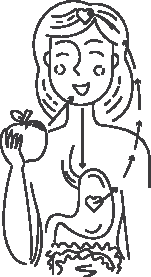
\includegraphics[scale=1.5]{willpower/ch4/12.pdf}
\end{figure}

\subsection*{Ліпастат}
У нашым арганізьме існуюць мэханізмы падтрыманьня пэўнага адсотку тлушчу незалежна ад ваганьняў каляражу. Калі мы больш зьелі, то падсьвядома і рухаемся больш, больш вытрачаем на тэрмагенэз\index{тэрмагенэз}. Гэты мэханізм, які фармаваўся на працягу мільёнаў гадоў, нашмат дакладнейшы за праграмы для падліку калёрыяў і да таго ж цалкам аўтаматызаваны. Наш мозг апрацоўвае мноства ўваходных зьвестак і прымае рашэньні, якія ўплываюць на нашы харчовыя паводзіны, сытасьць і апэтыт. Занадта смачная ежа, лішак сьвятла, стрэсу, зьмена долі тлушчу зьбіваюць наш ліпастат.

\infobox{Рэгулярныя эпізоды пераяданьня таксама могуць парушыць нармальную працу мэханізмаў насычэньня, таму нядзіўна, што наступствы навагодніх сьвятаў «вісяць» у~нас на баках да лета.}

Хранічнае запаленьне, напрыклад, вядзе да таго, што ў~гіпаталямусе зьмяняецца актыўнасьць нэўронаў, і яны пачынаюць выпрацоўваць больш гармонаў голаду. А калі разьвіваецца лептынарэзыстэнтнасьць\index{лептынарэзыстэнтнасьць}, то работа ліпастату зьмяняецца, чалавек пачынае думаць пра ежу, трызьніць ежай, захапляцца праглядам кулінарных шоў і набіраць вагу.

Калі ў~вас ёсьць выразныя харчовыя правілы, напрыклад, вы датрымліваецеся чыстых прамежкаў, то вы не марнуеце мэнтальную энэргію на барацьбу з~харчовымі спакусамі. Напрыклад, ідзяце вы паўз цукерню і адчуваеце спакусьлівы водар. Калі правілаў няма, вы пачынаеце думаць і сумнявацца, уключаць і хутка адключаць сілу волі.

\emph{Калі ў~спэктаклі на сьцяне вісіць стрэльба, то яна абавязкова стрэліць, а~калі ў~вас у~сумцы ляжыць баўнці, дык вы, ясная рэч, яго зьясьце і прыдумаеце потым сабе рацыянальнае апраўданьне для гэтага. Не спакушайце сябе дарма!}

Старажытныя інстынкты працуюць супраць нас: мы хочам выжыць і працягнуць род, і, калі раней набор вагі пры цяжарнасьці дапамагаў выжыць маці і дзіцяці, то сёньня атлусьценьне\index{атлусьценьне} павялічвае рызыкі для здароўя і зьмяншае фэртыльнасьць. Наш мозг заўсёды скануе прастору ў~пошуках калёрыяў, і найболей прывабна для яго выглядаюць прадукты, якія лёгка займець: анляйн-замова, хуткая дастаўка дадому, танная ежа, акцыі, зьніжкі, гатовая ежа, якая не патрабуе ані гатаваньня, ані нават жаваньня ці выкарыстаньня прыбораў, ежа з~высокай калярыйнай шчыльнасьцю. \textbf{Менавіта таму так важна есьці цэльную простую ежу: немагчыма атрымаць харчовую залежнасьць і пераядаць варанай рыбай і сырой салерай.}

Цэнтрам кантролю вагі, вядома, зьяўляецца кантроль энэргетычнага балянсу. Але для палягчэньня яго важна зьмяніць свае звычкі, рэжым харчаваньня, від прадуктаў так, каб паменшыць колькасьць чыньнікаў, якія павялічваюць апэтыт і пераяданьне, і павялічыць колькасьць чыньнікаў, якія павялічваюць сытасьць і зьніжаюць спажываньне калёрыяў. Выпрацаваўшы такія звычкі, мы зможам не пераядаць нават без штодзённага падліку калёрыяў.

\subsection*{Пытаньні і заданьні}

1. Вы перакусваеце? Падлічыце, колькі лішніх калёрыяў вы атрымліваеце выпадковымі перакусамі.

2. Як вы пераносіце пачуцьцё голаду?

3. На працягу аднаго тыдня падлічвайце свой сутачны каляраж і энэргетычны балянс.


\section{Падтрымка асяродзьдзя}

Наша цела хоча быць здаровым і супраціўляецца відавочнай шкодзе, але паступова гэтая сыстэма дае збой~--- з~розных прычынаў, пачынаючы ад амаль прымусовага закормліваньня з~самага дзяцінства, заканчваючы лішкам фастфуду\index{фастфуд}, рэклямы і высокім узроўнем стрэсу. 

\infobox{Няўжо мы вымушаныя ўвесь час змагацца з~сабой, валявым намаганьнем адводзяць вочы ад смачнай ежы? Наўрад ці гэта будзе эфэктыўна, бо нашая воля~--- канечны рэсурс.}

Вялікая колькасьць спэцыялістаў упэўненыя, што навучаньне падліку калёрыяў і іх штодзённы кантроль~--- аснова здаровага харчаваньня, а~людзі, якія ня могуць прытрымлівацца гэтай сыстэмы,~--- слабавольныя стварэньні. Але дасьледаваньні паказваюць, што нават тыя людзі, што лічаць калёрыі, робяць хібы, якія даходзяць да 25\,\% калярыйнасьці, пры гэтым падлічыць свой сапраўдны выдатак энэргіі вельмі цяжка. Дык што ж атрымліваецца~--- сыстэма добрая, а~людзі, якія не могуць схуднець на ёй,~--- дрэнныя!? Насамрэч усё крыху больш складана. 

\emph{Вядома, ня варта цалкам выключаць падлік калёрыяў: вы можаце палічыць свой каляраж на працягу аднаго-двух тыдняў, каб лепш арыентавацца ў~``лічбах'' таго, што вы зьядаеце.}

Мноства харчовых рашэньняў прымаецца несьвядома, і толькі потым мозг рацыяналізуе ўжо прынятае рашэньне. Падлік калёрыяў і плянаваньне рацыёну патрабуюць канцэнтрацыі і валявых рашэньняў, што цяжка для чалавека з~высокай працоўнай нагрузкай і ў~стане хранічнага стрэсу. Акрамя таго, важным зьяўляецца і кіраваньне голадам, бо тое харчаваньне, якое не забясьпечвае больш-менш прымальны ўзровень сытасьці, вырачанае на правал. 

Спалучэньне «пастаянны голад + стрэс» непазьбежна прывядзе да зрыву, за якім рушыць усьлед рыкашэтны набор вагі. \textbf{Таму варта ствараць такую сыстэму харчаваньня, якая б дазволіла зьменшыць колькасьць зьяданых калёрыяў без павышэньня пачуцьця голаду і затратаў на валявы самакантроль.}

\emph{«Я мяркую, што калі адзіны інструмэнт, які вы маеце,~--- малаток, то заманліва разглядаць усё як цьвікі», -- сказаў Маслоу. У дачыненьні да харчаваньня гэта канцэпцыя падліку калёрыяў. Зразумела, зьніжэньне каляражу~--- гэта эпіцэнтар правіла «еж менш, будзь танчэйшым, жыві даўжэй». Правіла адно, але шляхоў яго дасягненьня шмат. Напрыклад, для адной тэарэмы Піфагора вядома ня менш за 400 розных слушных доказаў. Так і для зьніжэньня колькасьці спажываных калёрыяў можа быць шмат спосабаў, у~тым ліку і тыя, дзе калёрыі лічыць ня трэба.}

У падліку калёрыяў ёсьць шэраг нэгатыўных аспэктаў: гэта складана рабіць на доўгатэрміновай аснове, бо патрабуе валявых сьвядомых намаганьняў, людзі схільныя да самападману, падлік калёрыяў правакуе абмежавальныя паводзіны і разлады харчовых паводзінаў, пастаянна пачуцьцё голаду вельмі дыскамфортнае. Калёрыі ежы замест крыніцы энэргіі становяцца пагрозай, і гэта не спрыяе нашаму псыхічнаму здароўю. Таму для кожнага канкрэтнага чалавека важна абраць найболей аптымальны для яго падыход да паніжэньня каляражу. Для кагосьці гэта будзе проста зьніжэньне стрэсу і трывогі.

\begin{figure}[ht!]
  \centering
  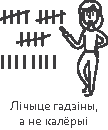
\includegraphics[scale=1.5]{willpower/ch4/13.pdf}
\end{figure}

Існуюць розныя прыёмы, кожны зь іх дае невялікі вынік, але ў~суме яны дзейнічаюць эфэктыўна~--- напрыклад, кіраваньне сытасьцю, стварэньне асяродзьдзя без харчовых трыгераў\index{трыгер}, мікрамэнэджмэнт харчаваньня, прыёмы гастрафізікі. Стварыўшы такую сыстэму, вы будзеце есьці менш, а~адчуваць сябе больш сытымі. Напрыклад, звужэньне харчовага акна да 6--8 гадзінаў ужо аўтаматычна прыводзіць да таго, што мы ямо на 500 ккал у~содні менш, а~выбар цэльнай ежы замест перапрацаванай~--- да зьніжэньня каляражу на супастаўнае значэньне пры захаваньні ранейшай сытасьці.

\subsection*{Харчовае ўстрыманьне}
Да ліку самых эфэктыўных стратэгіяў адносіцца звужэньне харчовага вакна і пэрыядычны фастынг\index{фастынг}, пра якія мы казалі вышэй. Лічым гадзіны, а~не калёрыі, і не абмяжоўваем сябе ў~ежы ў~вузкім харчовым вакне: такое абмежаваньне дазваляе зьменшыць колькасьць зьяданага.

\subsection*{Удзельная калярыйная шчыльнасьць}
Агульная ідэя~--- скарачаць колькасьць калярыйных прадуктаў, адначасова павялічваючы аб'ём малакалярыйных. Напрыклад, есьці ня проста крупы, а~іх сумесь з~гароднінай і зелянінай, заправіць салату кефірам або воцатам і да т.~п. Так мы будзем есьці больш па аб'ёме, а~дастатковы аб'ём ежы расьцягвае сьценкі страўніка, што стымулюе выдзяленьне гармонаў сытасьці.

\begin{figure}[ht!]
  \centering
  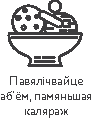
\includegraphics[scale=1.5]{willpower/ch4/14.pdf}
\end{figure}

\subsection*{Мяняйце прапорцыі прадуктаў}
Напрыклад, дзьве трэці агародніны і трэць крупаў на талерцы. Можна і перакінуць прапорцыі, зрабіць салату з~фасольлю, а~не фасолю, пасыпаную невялікай колькасьцю зеляніны. Вы можаце падлічыць усе свае прадукты за дзень і намаляваць сваю асабістую «прадуктовую талерку» для лепшага разуменьня, што і ў~якіх прапорцыях вы ясьце. 

\infobox{Прадукты з~больш высокай удзельнай шчыльнасьцю варта есьці самымі апошнімі падчас сталаваньня.}

\emph{Эфэктам насычэньня валодае і вада: 500\,мл вады, выпітыя перад прыёмам ежы, зьмяншаюць аб'ём зьедзенага на 22\,\%. А калі вы дадасьце ў~ваду імберац або мэнтол, гэта дасьць яшчэ мацнейшае насычэньне. Іншае дасьледаваньне паказала, што зьедзены першым суп памяншаў пачуцьцё голаду і колькасьць зьедзеных калёрыяў на 100\,ккал.}

\begin{figure}[ht!]
  \centering
  
\includegraphics[scale=1.5]{willpower/ch4/15.pdf}
\end{figure}

\subsection*{Кіраваньне голадам і сытасьцю}
Сытасьць~--- гэта зьнікненьне голаду, таму для таго, каб злавіць сытасьць, важна мець апэтыт перад ежай. Як толькі апэтыт зьнікае~--- гэта і ёсьць сапраўдны пункт сытасьці. Насычэньне~--- шматступенны працэс, дзе мы можам кіраваць кожным этапам: сэнсарнае насычэньне, мэханічнае, кішачнае, мазгавое, энэргетычнае.

\begin{figure}[ht!]
  \centering
  
\includegraphics[scale=1.5]{willpower/ch4/16.pdf}
\end{figure}

\textbf{Важна ў~кожны прыём ежы есьці ўволю, тады вы будзеце пачувацца сытымі да наступнага прыёму ежы.} Наступныя кампанэнты павялічваюць сытасьць, зьніжаюць голад і колькасьць зьедзенага: вада, клятчатка, цьвёрдасьць ежы (яе трэба жаваць), розныя спэцыі, фітанутрыенты, кіслы, горкі і перны смакі, пахі і да т.~п. Пах вельмі важны. Згадайце, якая нясмачная ежа, калі закладзены нос. Абавязкова нюхайце ежу перад тым, як яе зьесьці. Нават калі вы проста панюхаеце горкую чакаляду, гэта можа зьнізіць узровень гармону голаду грэліну. А наогул такія прадукты, як какава ці горкая чакаляда, імберац, чырвоны перац, памяншаюць апэтыт, павялічваюць сытасьць, зьніжаюць цягу да салодкага і могуць дапамагчы ў~пахудзеньні.

\emph{Для розных прадуктаў ёсьць табліцы індэксаў, якія ацэньваюць суадносіны калярыйнасьці і сытасьці. Напрыклад, сытасьць 100 грамаў курыцы і 250 грамаў пірага аднолькавая. Часам параўноўваюць сытасьць адносна белага хлеба, прымаючы яе за 100\,\%: тады рыба дае сытасьць 225\,\%, амлет 209\,\%, яблыкі 197\,\%, а~вось круасан 47\,\%, пончыкі 68\,\%, пірожнае 65\,\% і да т.~п. Наш мозг загадзя ацэньвае стравы, і мы несьвядома выбіраем той іх аб'ём, які забясьпечыць нам сытасьць,~--- гэта называецца «чаканая сытасьць страваў». Не выпадкова надзейнай «схэмай» для пахуданьня лічыцца «гародніна + рыба», бо яны выдатна насычаюць і дапамагаюць кантраляваць голад, перадухіляючы пераяданьне!}

Бабовыя, садавіна, гародніна, водарасьці, грыбы, цэльназерневае збожжа ўтрымоўваюць шмат клятчаткі, якая зьяўляецца магутным сродкам падтрыманьня сытасьці. Дасьледаваньні паказваюць, што даданьне бабовых можа павялічыць сытасьць на 31\,\% у~параўнаньні з~эквівалентнымі па макранутрыентах прадуктамі. Распушчальныя і глейкія тыпы клятчаткі, такія як пэктыны (яблык) і бэта-глюканы (авёс), даюць вялікую сытасьць: так, кожныя дадатковыя 14 грамаў клятчаткі на 10\,\% зьмяншаюць колькасьць зьяданых калёрыяў.

\begin{figure}[ht!]
  \centering
  
\includegraphics[scale=1.5]{willpower/ch4/17.pdf}
\end{figure}

\textbf{Падвышаюць апэтыт і пераяданьне} высокаглікемічныя вугляводы і рафінаваныя прадукты, якія ўтрымліваюць вялікую колькасьць стымулятараў апэтыту і малую~--- тармазоў: глутамат, узмацняльнікі смаку, араматызатары, фарбавальнікі~--- некалярыйны фарбавальнік можа на 13\,\% павялічыць колькасьць зьедзенага. Акрамя гэтага, яны яшчэ й вельмі калярыйныя, бо ўтрымоўваюць шмат даданага крухмалу, соі, тлушчу, цукру, солі і нізкае ўтрыманьне клятчаткі і бялку. Найбольш небясьпечная для нашай сыстэмы насычэньня камбінацыя цукар+тлушч. У прыродзе яна амаль не сустракаецца, але вось у~гатовых прадуктах харчаваньня~--- паўсюдна. Такая ненатуральная камбінацыя стымулюе пераяданьне і правакуе харчовую залежнасьць.

Уплываюць на апэтыт і іншыя чыньнікі, напрыклад, узровень фізычнай актыўнасьці, вячэрняе асьвятленьне, наяўнасьць сацыяльных кантактаў. Людзі, якія больш рухаюцца, адчуваюць сябе больш сытымі і менш ядуць, занадта яркае сьвятло ўвечары можа правакаваць начны апэтыт, а~самота ўзмацняе голад.

\begin{figure}[ht!]
  \centering
  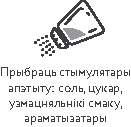
\includegraphics[scale=1.5]{willpower/ch4/18.pdf}
\end{figure}

\textbf{Бялок зьяўляецца адным з~магутных чыньнікаў насычэньня.} У дасьледаваньнях на жывёлах навукоўцы выявілі, што менавіта ваганьні бялку ў~дыеце ўплываюць на іх паводзіны. Гэтую зьяву назвалі гіпотэзай бялковага рычага: яе сутнасьць у~тым, што жывёлы імкнуцца ў~першую чаргу набраць неабходны мінімум бялку і толькі затым зважаюць на тлушчы і вугляводы. Патрэбны набор бялку прыкметна зьніжае апэтыт і абмяжоўвае далейшае пераяданьне. Матэматычная мадэль, якая апісвае ваганьні макранутрыентаў, пацвердзіла, што доля бялку ў~агульнай колькасьці калёрыяў у~розных людзей па ўсім сьвеце сапраўды вагаецца ў~вузкіх межах (каля 10--15\,\%), у~той час як прапорцыі тлушчаў і вугляводаў моцна вар'іруюцца. У паляўнічых-зьбіральнікаў сярэдняе ўтрыманьне бялку ў~рацыёне было дастаткова высокім~--- ад 20\,\% да 30\,\% ад агульнай каларыйнасьці.

\emph{Ідэя аб тым, што павелічэньне долі бялку дапаможа зьнізіць пераяданьне і будзе спрыяць пахудзеньню, здаецца заманлівай, але гэта занадта моцнае спрашчэньне. Шэраг дасьледаваньняў паказвае, што доля бялку ў~рацыёне мала адрозьніваецца ў~людзей з~атлусьценьнем\index{атлусьценьне} і без, і што ключавая роля ў~пахудзеньні належыць усё-ткі зьніжэньню колькасьці высокаглікемічных вугляводаў. Акрамя таго, высокабялковыя дыеты ў~доўгатэрміновай пэрспэктыве маюць шэраг нэгатыўных уласьцівасьцей.}

\textbf{Як жа можна выкарыстоўваць насычальную сілу бялковага рычага?} Важна есьці цэльныя бялковыя прадукты, а~ня іх камбінацыі з~вугляводамі і тлушчамі, накшталт гамбургера ці кашы зь мясам. Інакш для таго, каб ужыць неабходную колькасьць бялку, трэба будзе паралельна зьесьці шмат вугляводаў і тлушчаў. Па выніках дасьледаваньня, бялок з~рыбы прыцішае апэтыт мацней, чым зь ялавічыны, так што вядомая мудрасьць пра аптымальную дыету «рыба + гародніна» знаходзіць сваё пацьверджаньне.

Я ўжо пісаў вышэй: для таго каб днём апэтыт быў меншы, важна зьядаць шмат бялку на сьняданак. Дасьледаваньне паказала, што высокабялковы сьняданак на 51\,\% мацней прыцішае апэтыт, чым проста павелічэньне колькасьці бялку ў~рацыёне. Бялковы сьняданак, у~параўнаньні з~вугляводным, прыводзіць да на 65\,\% больш выяўленай страты масы цела пры пахудзеньні на працягу васьмі тыдняў дасьледаваньня.

\subsection*{Псыхалёгія харчаваньня}
Памяць, гіпакамп і колькасьць зьедзенай ежы шчыльна зьвязаныя паміж сабой. У выпадках рэтраграднай амнэзіі, калі чалавек забываецца на тое, што адбываецца зь ім, ён увесь час адчувае моцны голад і хоча есьці. Наш мозг плянуе каляраж, зыходзячы са стратэгічных мэтаў. Таму дакладная памяць аб тым, што вы зьелі сёньня, зьніжае колькасьць зьедзенага. А вось калі вы елі, адцягваючыся на тэлевізар ці інстаграм, то гэтая яда запомніцца дрэнна, і вы будзеце прыкметна пераядаць у~наступныя прыёмы ежы.

\emph{У дасьледаваньні ўдзельнікі ўяўлялі, што зьядаюць 3 ці 33 салодкіх дражэ, а~затым атрымлівалі міску зь імі. Тыя, хто ва ўяўленьні маляваў 33 дражэ, у~выніку зьядалі на 60\,\% менш. Так што нават візуалізацыя вялікай колькасьці ежы прывядзе да зьніжэньня аб'ёму фактычна зьедзенай ежы.}

\begin{figure*}[tb!]
  \centering
  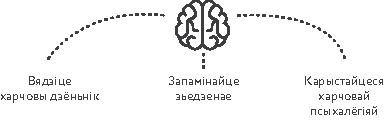
\includegraphics[scale=1.5]{willpower/ch4/19.pdf}
\end{figure*}

% ((вядзіце харчовы дзёньнік запамінайце зьедзенае карыстайцеся харчовай псыхалёгіяй))

\emph{У іншым дасьледаваньні паддосьледныя атрымлівалі малочны кактэйль аднолькавай калярыйнасьці 380 ккал, але з~рознымі этыкеткамі: на адных~--- з~калярыйнасьцю 140 ккал, на іншых~--- 620 ккал. Адзначыўшы зыходны ўзровень грэліну, вымералі яго пасьля прыёму напою. У тых, хто выпіў 620 ккал, грэлін рэзка ўпаў (зьніжэньне грэліну~--- гэта сыгнал сытасьці), у~тых, хто выпіў «дыетычныя» 140 ккал,~--- нічога не зьмянілася.}

\emph{Трэніраваць памяць і ўяўленьне~--- карысна і для фігуры. Калі сядаеце есьці, успомніце, што вы елі мінулым разам. Вядзіце харчовы дзёньнік~--- гэтыя запісы аўтаматычна зьніжаюць колькасьць зьедзенага. \textbf{Што практычнага мы можам засвоіць з~гэтых урокаў для сябе?}}

\subsection*{Паважайце ежу}
Калі мы сядаем за стол з~думкай «толькі б не памерці з~голаду ад гэтай травы», то ні задавальненьня, ні сытасьці не атрымаем. Калі ўспрымаем ежу з~удзячнасьцю і падзякай, калі ведаем, колькі ў~ёй вітамінаў, мінэралаў і карысных рэчываў, то гэтыя веды і павага трансфармуюцца ў~сытасьць і задавальненьне. 

\infobox{Думайце пра ежу як пра крыніцу энэргіі. Бо гэта сапраўды так: лічаныя месяцы таму энэргія, заключаная ў~хімічных сувязях вашай брокалі, была фатонамі, якія нарадзіліся ў~тэрмаядзерных сонечных рэакцыях. Ведайце і паважайце ежу, і яна адкажа вам узаемнасьцю!}

\emph{Згадваю свае перамовы з~адной кавярняй. Ідэя была даць стравам назвы, якія гучаць цудоўна, каб пры замове госьць атрымліваў аркуш з~падрабязным апісаньнем інгрэдыентаў, іх карысьці, уплыву на арганізм, працэсу гатаваньня. Чытаньне запускае мазгавую стадыю страваваньня, дазваляе весялей прабавіць час, чакаючы страву, пашырае спэктар харчовых ведаў. Такія назвы, як «далікатэсная гародніна на грылі беражлівага гатаваньня па рэцэптах праванскай кухні», павялічваюць колькасьць атрыманага «некалярыйнага» задавальненьня і насычэньня ад ежы. Пры гэтым ёсьць плюсы для рэстарана: продажы растуць, рэйтынг установы павялічваецца, кліенты гатовыя плаціць больш.}

Дома мы заўсёды даём заданьне дзецям назваць усе інгрэдыенты стравы і даць ёй «смачную» назву. Рабіце так і самі~--- і ежа будзе смачнейшай. А вось у~рэстаране будзьце больш уважлівымі да такіх назваў, яны могуць уводзіць вас у~зман!

\subsection*{Стварэньне асяродзьдзя}
Ваша непасрэднае асяродзьдзе істотна на вас уплывае: чым больш у~вас сяброў з~атлусьценьнем\index{атлусьценьне}, тым вышэйшая рызыка набраць вагу і для вас. І наадварот, павелічэньне колькасьці людзей са звычайнай вагой вакол вас павялічвае і вашыя шанцы мець нармальную вагу. Пераезд у~раён з~больш высокім узроўнем даходу зьніжае рызыку атлусьценьня. Цікава, але ўплывае нават блізкасьць крамаў: чым бліжэй яны да доду, тым вышэйшая рызыка атлусьценьня\index{атлусьценьне}. Усё гэта яшчэ раз нагадвае нам, што велізарную колькасьць харчовых рашэньняў мы прымаем несьвядома, таму так важна ствараць асяродзьдзе, якое нас падтрымлівае: \textbf{натхняцца сваімі мэтамі, камунікаваць з~аднадумцамі і падтрымліваць правільны набор прадуктаў на кухні.}

Не трымайце ежу навідавоку, не захоўвайце дома снэкі і алькаголь\index{алькаголь}, нават пад маркай «для гасьцей». Раскладзіце правільна ежу на паліцах і ў~лядоўні: тое, што вы хочаце есьці часьцей, хай ляжыць на ўзроўні вачэй і ў~празрыстых кантэйнэрах, тое, што хочаце ёсьць радзей,~--- далей ад вачэй і ў~непразрыстых кантэйнэрах з~накрыўкамі. Не захоўвайце на кухні паўфабрыкаты, а~майце запас замарожанай гародніны, рыбы і яек. Выкладвайце на стол ня печыва з~цукеркамі, а~сырую парэзаную гародніну, гарэхі і несалодкую садавіну. 

\infobox{Многія людзі ядуць на аўтамаце: калі бачаць, будуць есьці, пакуль ежа не скончыцца. Эфэктыўна будзе проста прыбраць спакусу з~поля зроку і ўласнай кухні. Чым менш будзе правакацый, тым радзей вы ім будзеце паддавацца.}

\textbf{Геданістычнае пераяданьне~---} яда для задавальненьня, а~абжорства, нагадаю, гэта сьмяротны грэх. Атрымліваць задавальненьне ад наталеньня голаду~--- цалкам натуральна, але часта людзі кампэнсуюць ежай недахоп камунікацыі, хобі, шпацыраў ды іншых простых чалавечых радасьцяў. Для таго каб паслабіць гэты патэрн, варта атрымліваць больш задавальненьня ад працэсу яды і адначасова ад іншых сфэраў свайго жыцьця. Ежце з~задавальненьнем, а~ня ежце дзеля задавальненьня!

\textbf{Вы можаце выбіраць любімыя прадукты і даваць яркія назвы стравам, і пры гэтым заплянаваць сабе на вечар прыемную справу~--- тады вы зьясьце на вячэру меней!} Калі ў~вас ёсьць залежнасьць ад ежы, то рэзкая адмова ад усяго «смачнага» можа прывесьці вас да зрыву, таму кампэнсуйце калярыйны дафамін некалярыйным.

\emph{Радасьць валодае тлушчаспаляльным эфэктам: мае назіраньні паказваюць, што займальнае хобі ці закаханасьць могуць лёгка пазбавіць чалавека ад лішніх кіляграмаў. Шэраг дасьледаваньняў зьвязвалі зьніжэньне ўзроўню дафаміну і атлусьценьне\index{атлусьценьне}~--- разглядаліся вэрсіі зьніжэньня рухальнай актыўнасьці і адчувальнасьці да інсуліну.}

\textbf{Стрэсавае пераяданьне~---} частая зьява. Існуе анекдот, што ўсе хваробы ад нэрваў і пераяданьня, таму ня трэба перажываць і перажыраць. Навукоўцы высьветлілі, што нізкі сацыяльны статус, нявызначанасьць, беднасьць павялічваюць пераяданьне. Нават аднаразовы стрэс прыводзіць да таго, што пасьля яго паддосьлеьныя зьядаюць на 22\,\% калёрыяў больш. \textbf{Што яшчэ горш, пераяданьне на тле стрэсу вядзе да павелічэньнянію менавіта вісцэральнага тлушчу, самага небясьпечнага для здароўя.}

Стрэс, роўна як і стома, алькаголь\index{алькаголь}, сьпешка, забароны, недасып, зьніжае самакантроль і павялічвае імпульсіўнасьць, што робіць нас больш адчувальнымі да вонкавых харчовых сыгналаў. Невыпадкова раней рэкляма аднаго вядомага напою з~кафэінам і цукрам мела побач з~рэклямным стэндам пункт продажу гэтага напою.

\subsection*{Талерка і прыборы} 
Кажуць, што пад дажджом суп можна есьці вечна. У адным дасьледаваньні да талеркі паддосьледных правялі шланг і ўвесь час папаўнялі міску супу. Гэтыя людзі зьелі на 73\,\% больш, чым тыя, хто наліваў сабе суп самастойна. Цікава, што ўдзельнікі, якія зьелі больш, не адчувалі сябе больш сытымі. 

\infobox{Гэтую зьяву называюць «эфэкт пустой талеркі», калі мы схільныя зьядаць усё, што сабе паклалі. Таму важна накладваць дзьве траціны таго, што вы хочаце зьесьці, або выпрацаваць звычку не даядаць хаця б трошкі.}

Памер мае значэньне: выкарыстоўваючы аптычныя ілюзіі, можна паўплываць на ўспрыманьне колькасьці ежы. Рэч у~тым, што наш мозг ацэньвае колькасьць ежы яшчэ да таго, як мы пачалі есьці. Мы зьядаем «дастаткова» менавіта на думку мозгу.

\emph{Ілюзія Дэльбэфа~--- пра ўплыў кантэксту на ўспрыманьне. У клясычным яе варыянце ёсьць два колы аднолькавага памеру, але адно зь іх у~кольцы вялікага дыямэтру, а~другое~--- маленькага. Другое кола візуальна здаецца нам большым за першае, хоць насамрэч яны роўныя. Чым большая ваша талерка, тым меншай вашаму мозгу здаецца порцыя і тым больш вы ясьце.}

Чым кантрасьнейшая талерка ў~адносінах да ежы, тым менш мы накладваем: удзельнікі дасьледаваньня, якія выбіраюць пасту на белай талерцы, кладуць сабе на 30\,\% больш, чым удзельнікі з~чырвонай талеркай. Чым кантрасьнейшы абрус у~адносінах да талеркі, тым менш мы накладваем. Пры гэтым чым вышэйшы ўзровень адукацыі і чым больш уважлівы ўдзельнік, тым менш ён схільны да гэтай ілюзіі.

\emph{Памер і колер маюць значэньне. Калі сэрвіраваць напоі ў~высокіх і тонкіх шклянках, удзельнікі вып'юць на 20\,\% менш. Выкарыстаньне лыжак вялікага памеру прыводзіць да павелічэньня зьедзенага на 14,5\,\%, а~вось цяжкія талеркі, цяжкія прыборы, цяжкія шклянкі вядуць да памяншэньня зьедзенага. Падыграйце вашаму мозгу: больш салаты вы зьясьце зь вялікай зялёнай талеркі, а~менш пасты ці рысу~--- зь невялікай чорнай ці чырвонай.}

Сіні і блакітны колеры талеркі мацней за ўсё зьніжаюць апэтыт і памяншаюць колькасьць зьедзенага на 15\,\%. Кава ў~сініх і шкляных кубках здаецца менш горкай, а~вось белыя кубкі падсьвядома павялічваюць яе гаркату. Гарбата ў~празрыстым посудзе здаецца менш гарачай, гарбата зь лімонам духмянейшая ў~жоўтым кубку, а~напоі ў~сініх кубках лепей спаталяюць смагу. 

Салодкія дэсэрты на белай талерцы здаюцца на 7\,\% саладзейшымі і на 13\,\% смачнейшымі, чым на чорнай. З чырвонай талеркі мы зьядаем менш дэсертаў, а~з чырвоных кубкаў выпіваем менш салодкіх напояў, у~параўнаньні зь сінімі ці белымі. Паэкспэрымэнтуйце.

\subsection*{Пытаньні і заданьні}

1. Якія прадукты правакуюць пераяданьне?

2. Якія эмоцыі, паводзіны, самаадчуваньне падштурхоўваюць вас да пераяданьня?

3. Якія прадукты насычаюць вас надоўга?


\section{Структура цела}

Традыцыйна мы вымяраем сваю вагу і індэкс масы цела (ІМТ). Гэты індэкс састарэлы і часьцяком зьяўляецца толькі крыніцай стрэсу. Чаму? ІМТ~--- вельмі грубы ўсярэднены паказьнік, які выкарыстоўваецца для дасьледаваньня вялікіх груп людзей, пры гэтым сьціраюцца іх індывідуальныя адрозьненьні. Для пэрсанальнай ацэнкі гэты індэкс выкарыстоўваць нельга: рэч у~тым, што з~пункту гледжаньня ІМТ няма падзелу паміж цяглічнай і тлушчавай тканкай. Чалавек зь лішкамі тлушчу і атлет з~разьвітой мускулатурай будуць мець аднолькавы ІМТ, а~адначасовая страта цягліц і павелічэньне тлушчу зь цягам часу можа нават не адбіцца на ІМТ. 

\infobox{Наш мозг ці, напрыклад, ныркі ня могуць заўважна мяняць сваю вагу на працягу жыцьця. Толькі тлушчавая тканка, цяглічная і колькасьць вадкасьці (водна-солевы балянс) даюць ваганьні вагі.}

\textbf{Калі гаворка ідзе пра тлушчавую масу,} трэба ўлічваць дзьве яе галоўныя разнавіднасьці~--- падскурны і вісцэральны тлушч. Вісцэральны тлушч разьмяшчаецца ў~поласьцях цела і вельмі небясьпечны для здароўя, пры гэтым яго цяжка выявіць. Падскурны тлушч разьмяшчаецца ў~падскурна-тлушчавай клятчатцы, для яго мае значэньне ня толькі колькасьць, але і характар разьмеркаваньня. Разьмеркаваньне залежыць як ад генэтычных асаблівасьцяў, так і ад гарманальнага статуту. Напрыклад, «ніжні» тлушч на ягадзіцах валодае ахоўным дзеяньнем, а~вось павышэньне тлушчавай праслойкі па контуры твару (паўмесяцовы твар) можа быць зьвязана зь лішкам картызолу. Характар разьмеркаваньня тлушчавай тканкі не залежыць ад велічыні ІМТ.

\emph{Праведзеныя дасьледаваньні на сумаістах паказалі, што нават у~вельмі тоўстых, але фізычна актыўных спартсмэнаў назіраецца добрая адчувальнасьць да інсуліну, а~вось у~былых сумаістаў адчувальнасьць ужо горшая~--- і больш вісцэральнага тлушчу.}

\textbf{Колькасьць цяглічнай масы~---} таксама вельмі важны паказьнік здароўя чалавека. Чым больш цягліцаў, тым менш рызыкаў для здароўя і даўжэйшая працягласьць жыцьця. Праблема ў~тым, што з~узростам ахоп канцавінаў можа асабліва не мяняцца: цягліцы замяшчаюцца тлушчам, і чалавек гэтага не заўважае. \textbf{Адыліж страта цягліц (саркапэнія\index{саркапэнія})~--- гэта адна з~самых сур'ёзных, але разам з~тым цалкам перадухільных пагроз для здароўя.}

Для ацэнкі здароўя трэба дакладна ацаніць колькасьць і разьмеркаваньне кожнага віду тлушчавай тканкі, іх суадносіны і колькасьць цягліц. Для зручнасьці давайце ўявім, што тлушч і цягліцы канкуруюць за пажыўныя рэчывы, якія знаходзяцца ў~крыві. Калі перавагі мае тлушч, то энэргія ідзе туды, цягліцы~--- да цягліц. Перапаўненьне тлушчавых клетак узмацняе вылучэньне супрацьзапаленчых малекул і павялічвае рызыкі для здароўя. Атрымліваецца, што нам трэба стаць цяглічна-дамінантнымі. 

\textbf{Недасып дае фору тлушчу:} пры недастатковай колькасьці сну цягліцы горш паглынаюць глюкозу, а~тлушч лепш. А вось рэгулярныя трэніроўкі на працягу паўгода прыводзяць да зьмены актыўнасьці генаў тлушчавай тканіны, і яны пачынаюць меней запасіць тлушч. 

Такім чынам, здаровы лад жыцьця яшчэ і ў~тым, каб даць перавагі цягліцам, і дасягаецца гэта сыстэмным працяглым падыходам. 

\emph{А што дамінуе ў~вас?}

\subsection*{Структура цела} 
Пры адной і той жа вазе не заўсёды можа быць аднолькавая структура цела. Як я кажу на курсах, «усё роўна, тоўсты ты ці худы, галоўнае~--- каб ня тлусты». Што гэта значыць? Людзі са звычайнай вагай могуць мець лішак вісцэральнага або агульнага тлушчу (больш тлушчу і менш цягліц), што павялічвае іх рызыкі для здароўя.

\emph{У сярэднім ад 45\,\% жанчынаў і 60\,\% мужчынаў з~нармальным ІМТ маюць лішак вісцэральнага тлушчу, да 10\,\% мужчынаў і жанчынаў маюць выяўлены лішак вісцэральнага тлушчу. Нават худыя мадэлі могуць мець яго лішак. Такі стан называецца «худы тлусты», або TOFI~--- Thin Outside, Fat Inside.}

\textbf{Тофі~--- гэта як чалавек-бомба: праз нармальную вагу ён нават не падазрае, што яму нешта пагражае.} Пры гэтым над ім «навісаюць» усе праявы мэтабалічнага сындрому: артэрыяльная гіпэртэнзія\index{артэрыяльная гіпэртэнзія}, цукровы дыябэт\index{дыябэт}, сардэчна-сасудзістыя захворваньні\index{сардэчна-сасудзістыя захворваньні}, рак, дэпрэсіі\index{дэпрэсія} і інш. Дасьледаваньні паказалі, што 22\,\% мужчынаў і 8\,\% жанчынаў мелі лішак вісцэральнага тлушчу нават пры нармальным аб'ёме таліі. МРТ паказвае значныя ваганьні вісцэральнага тлушчу: у~двух людзей аднаго ўзросту, полу, росту, масы цела вісцэральны тлушч складае ад 5,86 да 1,65 літраў. Значная розьніца, праўда? Важна, што ў~такіх людзей значна павышаныя рызыкі для здароўя і ёсьць зьмены ў~аналізах: у~10--27\,\% асобаў са звычайнай масай цела сустракаюцца інсулінарэзістэнтнасьць і дысьліпідэмія.

Адваротны стан «тоўсты ня тлусты»~--- гэта FOTI~--- Fat Outside, Thin Inside, або мэтабалічна здаровае атлусьценьне\index{атлусьценьне}. Ад 10 да 40\,\% пацыентаў маюць пры лішку вагі нармальныя паказьнікі вугляводнага абмену, ліпіднага профілю, артэрыяльнага ціску, узроўню глюкозы, С-рэактыўнага бялку і адчувальнасьці да інсуліну. Але лічыцца, што пры ІМТ > 30\,кг/м${}^2$ рэальная распаўсюджанасьць гэтага стану ня больш за 5--15\,\%. Пры дасьледаваньнях у~такіх людзей няма лішку вісцэральнага тлушчу, а~лішняя вага ў~іх~--- за кошт падскурнага. Таксама яны захоўваюць высокі ўзровень фізычнай актыўнасьці.

\emph{Аднак вага ня можа расьці бясконца: дасьледаваньне блізьнятаў давяло, што пры дасягненьні 20\,\% тлушчу ў~мужчынаў і 39\,\% у~жанчынаў вісцэральны тлушч пачынае актыўна расьці. Таму мужчынам нават пры нармальных аналізах ня варта мець працэнт тлушчу вышэй за 15\,\%.}

\textbf{Залішняя вага~---} гэта ня проста касмэтычны недахоп, гэта сур'ёзнае павелічэньне рызыкі сардэчна-сасудзістых захворваньняў\index{сардэчна-сасудзістыя захворваньні}, дыябэту\index{дыябэт}, дэпрэсіі\index{дэпрэсія}, пухлінавых захворваньняў. Напрыклад, у~пажылых жанчынаў нават зь невялікім атлусьценьнем\index{атлусьценьне} рызыка раку маткі ў~10 разоў вышэй, чым пры нармальнай вазе. 

\infobox{Выяўнае атлусьценьне\index{атлусьценьне} скарачае працягласьць жыцьця да 9 гадоў. Кожны кіляграм, які вы скінеце, падаўжае ваша жыцьцё на 3--4 месяцы.}

Падабаецца нам гэта ці не, але цяпер структура цела зьяўляецца адным з~ключавых паказьнікаў сацыяльнага статусу чалавека. Успрыманьне статусу адбываецца на падкорцы, літаральна ў~першыя сэкунды знаёмства, а~ад ацэнкі статусу залежыць і камунікацыя, і разьмеркаваньне рэсурсаў. Дык вось, кожны лішні кіляграм вагі ў~сярэднім адымае ад зарплаты 1\,\%, незалежна ад полу, групы, сацыяльнага становішча. Самае непрыемнае, што праблема можа пачынацца ўжо ў~дзяцінстве. Дзеці, якія пакутавалі ад атлусьценьня\index{атлусьценьне}, пасталеўшы, атрымліваюць заробак на 18\,\% менш, проста поўныя~--- на 4\,\% менш. Гэта зьвязана з~тым, што яны атрымліваюць менш навыкаў, чым аднагодкі.

\textbf{Вісцэральны тлушч.} У 1947 годзе прафэсар Жан Ваг апублікаваў работу, дзе адзначыў, што рызыка гіпэртэнзіі\index{гіпэртэнзія}, ССЗ, падагры, дыябэту\index{дыябэт} залежыць ня столькі ад масы цела, колькі ад разьмеркаваньня тлушчу, і можа сустракацца ў~пацыентаў са звычайнай масай цела. Пасьля было ўстаноўлена, што менавіта вісцэральны тлушч~--- прычына разьвіцьця многіх захворваньняў, і што залішняя колькасьць вісцэральнага тлушчу можа быць і ў~худых, і ў~тоўстых. Вісцэральны тлушч больш супрацьзапаленчы, больш інэрваваны, мае больш высокі ўзровень ліполізу, уплывае на ўзровень сыстэмных гармонаў: лептыну, адыпанэктыну, палавыя гармоны. Застаецца пытаньне: чаму ён усё ж узьнікае?

\subsection*{Існуе некалькі тэорый, чаму расьце вісцэральны тлушч}
Першая~--- гэта «\textbf{перапаўненьне}», калі нарастае інсулінарэзістэнтнасьць печані, цягліц, тлушчавай тканіны, і тлушч адкладаецца ў~«эктапічных» месцах: сальнік, печань, цягліцы, падстраўніца і інш. А яго адрозныя ад падскурнага тлушчу ўласьцівасьці тлумачацца нетыповай лакалізацыяй. У гэтым меркаваньні ёсьць рацыянальнае зерне: «мэтабалічна здаровае атлусьценьне\index{атлусьценьне}» ня можа быць якім заўгодна вялікім: калі перавышэньне масы цела большае за 15\,\%, то вісцэральны тлушч пачынае павялічвацца. Аднак гэта не тлумачыць фэномэну «худых тлустых».

Другая тэорыя пра тое, што \textbf{вісцэральны тлушч пачынае расьці пры гарманальных парушэньнях}: лептынрэзістэнтнасьці\index{лептынарэзыстэнтнасьць} і інсулінрэзістэнтнасьці. Бо лептын, акрамя ўсё іншага, яшчэ і «рэгуліроўшчык» тлушчу, які ўплывае на характар яго адкладаў. Свой унёсак робіць парушэньне работы палавых гармонаў і картызол.

\textbf{Схільнасьць менавіта да вісцэральнага атлусьценьня\index{атлусьценьне} часьцей выяўляецца ў~мужчынаў, асабліва пры недасыпе і хранічным стрэсе.} У вісцэральных тлушчавых клетках больш рэцэптараў да картызолу, таму пры стрэсе яны растуць хутчэй за ўсё. Картызол павялічвае тлушч у~жываце, верхняй палове цела і менш за ўсё~--- у~нагах. Дэфіцыт тэстастэрону, які бывае пры стрэсе, пагаршае працэс. А чым шырэйшая талія і больш вісцэральнага тлушчу, тым меншы ўзровень тэстэстэрону.

Трэцяя, эвалюцыйная тэорыя тлумачыць унікальныя ўласьцівасьці вісцэральнага тлушчу праз \textbf{імуналагічную функцыю сальніка}. Сальнік~--- гэта зморшчына вісцэральнай брушыны, якая грае важную ролю ў~імунітэце~--- яна фільтруе кроў ад кішачніка. Імунныя клеткі сальніка адрозьніваюцца больш выяўленым тлушчавым абменам і высокай супрацьзапаленчай актыўнасьцю. І гэта нядзіўна, бо ў~кішачніку велізарная колькасьць антыгенаў! Сальнік называюць «паліцэйскім жывата»~--- ён можа абараняць ад запаленьня органы і нават стрымліваць распаўсюджваньне запаленьня па брушной поласьці. Такія ўласьцівасьці сальніка дапамагалі ў~асяродзьдзі з~вялікай колькасьцю кішачных інфэкцыяў.

\infobox{Што адбываецца цяпер, у~часы лепшай гігіены і меншай разнастайнасьці мікрафлёры? Запаленьне ў~кішачніку першапачаткова выклікаюць не мікробы, а~нездаровае харчаваньне.}

Канцэнтраваныя насычаныя тлушчы, фруктоза, высокаканцэнтраваныя вугляводы нэгатыўна ўплываюць на мікрафлёру, што прыводзіць да разьвіцьця постпрандыяльнай «мэтабалічнай эндатаксэміі», якая выяўляецца ў~павышэньні ўзроўню цыркуляцыі ў~крыві ліпаполіцукрыду і іншых запаленчых маркераў на працягу пяці гадзінаў пасьля яды. Звярніце ўвагу, што вінаватыя не вугляводы самі па сабе, а~іх удзельная калярыйная шчыльнасьць.

Такім чынам, падвышаная актыўнасьць сальніка на тле хранічнага запаленьня прыводзіць да дэкампэнсацыі яго ахоўнай функцыі, утвараючы заганнае кола: больш запаленьня~--- больш вісцэральнага тлушчу~--- больш запаленьня.

Колькасьць тлушчавай тканкі \textbf{не зададзеная генэтычна}. Яна рэдка фармуецца да нараджэньня і яе колькасьць малая да падлеткавага ўзросту. Але пры наборы тлушчу больш за 20\,\% у~мужчынаў, 39\,\% у~жанчынаў вісцэральная тканка пачынае моцна расьці, а~недасып, стрэс і зьніжэньне тэстастэрону павялічваюць яе ўзровень. Пры розных экстрэмальных «сушках» можна зьнізіць колькасьць падскурнага тлушчу, але больш устойлівы вісцэральны тлушч застаецца~--- успомніце атлетаў з~выпнутымі жыватамі.

\textbf{Менавіта зьніжэньне вісцэральнага тлушчу, а~ня проста схудненьне, зьніжае рызыку для здароўя.} Чым меней тлушчу ў~лёгкіх, тым лягчэйшае цячэньне астмы\index{астма}; чым меней тлушчу ў~падстраўніцы, тым лепшая адчувальнасьць да інсуліну; чым меней тлушчу ў~печані, тым лепей усяму арганізму. Вісцэральнае схудненьне~--- гэта самае здаровае схудненьне: зьмена харчаваньня, добры сон, фізычная актыўнасьць.

\subsection*{Вісцэральны тлушч}
Вісцэральны тлушч і агульны тлушч можна вымяраць рознымі спосабамі. Самы дакладны зь іх~--- гэта рэнтгенаўскае вымярэньне структуры цела, дзе можна ацаніць тлушчавую, цяглічную і касьцяную тканкі (DEXA). Але для паўсядзённага выкарыстаньня добра пасуе і антрапамэтрыя, і зьмешаныя спосабы, а~таксама УГД.

Для вымярэньняў вам спатрэбіцца сантымэтровая стужка і паўгадзіны часу. Рэкамэндуецца праводзіць такія вымярэньні раз на адзін-два тыдні.

\textbf{Абхоп таліі.} Вымерайце абхоп таліі з~дапамогай мернай стужкі без адзеньня. Акружнасьць таліі павінна быць вымераная пасярэдзіне паміж ніжнім краем ніжняга рабра і вяршыняй падуздышнага грэбеня (верхняя костка таза, яе відаць у~нас збоку). Пастаўце ногі разам, рукі расстаўце ўбакі, дыхайце спакойна, вымярайце ў~канцы выдыху. Кожны замер паўтарайце двойчы, і калі паміж імі розьніца ў~сантымэтар, то бярыце сярэдні вынік.

\textbf{Для мужчынаў: норма~--- 94\,см, павышаны паказьнік~--- да 102\,см, звыш 102\,см~--- крытычны паказьнік.}

\textbf{Для жанчынаў: норма~--- да 80\,см, павышаны паказьнік~--- да 84\,см, звыш 88\,см~--- высокая рызыка для здароўя.}

Чым шырэйшая талія, тым большая рызыка разьвіцьця хваробаў сэрца, палавой сыстэмы, раку. Кожныя 5 сантымэтраў на таліі павялічваюць рызыку заўчаснае сьмерці на 17\,\%. Нават невялікае зьмяншэньне таліі карыснае для здароўя.

\textbf{Абхоп сьцёгнаў.} Вымерайце з~дапамогай мернай стужкі акружнасьць сьцёгнаў у~самым шырокім месцы (ніжэй за вялікія сьцегнавыя бугры). 

\textbf{Сярэднія значэньні: 90--107\,см~--- мужчынскія сьцёгны, 90--110\,см~--- жаночыя сьцёгны.}

Занадта вузкія сьцёгны ў~жанчынаў павялічваюць рызыку дыябэту\index{дыябэт}, гіпэртэнзіі\index{гіпэртэнзія} і жоўцекамянёвай хваробы\index{жоўцекамянёвая хвароба}\index{хвароба!жоўцекамянёвая}. Нармальныя памеры ягадзіц зьвязаныя зь лепшым ліпідным профілем і меншай рызыкай шэрагу захворваньняў, ад сардэчна-сасудзістых да некаторых відаў раку. Гэтая сувязь больш характэрная для жанчынаў, чым для мужчынаў. Памер ягадзіц залежыць як ад разьвіцьця цягліц, так і ад тыпу адкладу тлушчу.

\textbf{Суадносіны талія-сьцёгны.}~\nopagebreak[4]

\textbf{Для мужчын: норма 0,9 (0,88--0,92), павышаны паказьнік~--- 0,92--1,0, больш за 1,0~--- атлусьценьне\index{атлусьценьне}.} 

\textbf{Для жанчын: норма 0,7 (0,68--0,77), павышаны паказьнік~--- 0,75--0,85, больш за 0,85~--- атлусьценьне\index{атлусьценьне}.}

Гэты паказьнік зьвязаны зь нізкай рызыкай разьвіцьця дыябэту, сардэчна-сасудзістых захворваньняў\index{сардэчна-сасудзістыя захворваньні} і гармон-залежных ракаў (у жанчынаў яечнікаў і грудзей, у~мужчынаў~--- падкарэньніцы), з~нармальнай фэртыльнасьцю і большай прывабнасьцю.

\textbf{АBSI індэкс} (\url{www.absicalculator.eu}). Індэкс формы цела паказвае адносіны паміж аб'ёмам таліі, ростам і вагой. Формула складаная, скарыстаемся калькулятарам, які ёсьць на сайце. Акрамя лічбаў, гэты індэкс яшчэ дае і ацэнку рызыкаў: чым вышэй лічба, тым вышэй рызыка хваробаў. 

\emph{У мяне ён роўны 0,76. Гэтая лічба азначае, што ў~мяне рызыка хваробаў меншая, чым у~сярэднім (сярэдняя рызыка = 1).}

\textbf{Акружнасьць шыі.} Вымерайце з~дапамогай мернай стужкі акружнасьць шыі ў~самым вузкім месцы. Звычайна акружнасьць шыі вымяраюць паміж сярэднім шыйным пазванком і сярэдзінай шыі сьпераду крыху ніжэй за выступ гартані. 

\textbf{Для мужчын: оптымум~--- да 35,5\,см, норма~--- да 40\,см, павышаны паказьнік~--- ад 45\,см.} 

\textbf{Для жанчын: оптымум~--- менш за 32\,см, норма~--- да 34,5\,см, павышаны паказьнік~--- 40\,см.}

Аптымальны (нармальны) абхоп шыі~--- паказьнік нізкае рызыкі мэтабалічных парушэньняў. Чым таўсьцейшая шыя, тым ніжэйшы ўзровень «добрага» халестэрыну і горшая адчувальнасьць да інсуліну, мацнейшая рызыка мэтабалічных парушэньняў, падвышанага ціску і рызыкі апноэ\index{апноэ}. 

\emph{Павелічэньне абхопу шыі ў~спартоўцаў, якія прыцэльна прымяняюць практыкаваньні для яе ўмацаваньня, не зьвязаная з~ростам рызыкі.}

\textbf{Суадносіны рост-талія.} Для гэтага абхоп жывата ў~см дзеляць на рост у~см. Можна зваротным спосабам разьлічыць ідэальную талію для дадзенага росту і вылічыць, колькі сантымэтраў трэба прыбраць для дасягненьня нормы. 

\textbf{Паказьнікі: 0,40--0,48~--- норма, 0,48--0,56~--- павышаны паказьнік, больш за 0,57~--- крытычна высокая рызыка мэтабалічных парушэньняў.}

\textbf{Вышыня жывата.} Вышыня жывата~--- гэта найменшая адлегласьць паміж двума гарызанталямі: той, якая ляжыць на паверхні жывата, і той, якая датыкаецца пазванка сьпіны. Вымяраць трэба, прыціснуўшыся сьпінай да падлогі і сагнуўшы ногі ў~каленях, на ўзроўні крыжа. Норма~--- да 25 сантыметраў. Вышыня жывата больш за 25\,см~--- гэта рызыка разьвіцьця хваробы Альцгаймэра\index{хвароба!Альцгаймэра}.

\textbf{Інструмэнтальныя і лябараторныя мэтады.} Залаты стандарт ацэнкі структуры цела~--- гэта \textbf{DEXA-сканаваньне} (Dual-Energy X-Ray Absorptiometry). Але гэта дорага, зьвязана з~апраменьваньнем і не заўсёды даступна для ацэнкі дынамікі. 

Вымярэньне біяэлектрычнага супраціву (біяімпэданс) дае памылкі да 10\,\% пры параўнаньні з~DEXA. Чым менш электродаў, тым горшая дакладнасьць вымярэньня, але шалі з~8 электродамі паказваюць досыць высокую дакладнасьць, да 94\,\% карэляцыі з~DEXA.

Біяімпэданс карысны, калі адсочваць дынаміку на адным апараце з~аднолькавымі ўмовамі, але чым мацней ваш целасклад адрозьніваецца ад сярэдніх значэньняў, тым вышэйшай будзе яго памылка. У худых біяімпэданс пераацэньвае сухую масу цела і недаацэньвае яе ў~поўных.

\emph{На біяімпэданс уплываюць і ўмовы яго правядзеньня. Так, нават невялікае абязводжваньне на 5\,кг прыніжае сухую масу цела і завышае ўтрыманьне тлушчу, прыём ежы можа завысіць утрыманьне тлушчу на 4,2\,\%, фізычная актыўнасьць нават за 2 гадзіны да зьмены можа прывесьці да пераацэнкі сухой масы цела да 12\,кг.}

\textbf{Ультрагукавое дасьледаваньне} можа ацаніць шэраг маркераў вісцэральнага атлусьценьня\index{атлусьценьне}. 

Спачатку робім дасьледаваньне печані: лінейныя памеры, прыкметы тлушчавага гепатозу, стан жоўцевага пухіра.

Затым вымяраем таўшчыню эпікардыяльнага тлушчу (рызыкі растуць пры лічбе больш за 5\,мм), колькасьць якога карэлюе з~узроўнем вісцэральнага тлушчу, і таўшчыню пэрыкардыяльнага тлушчу (сардэчныя рызыкі).

Пасьля чаго вымяраем адлегласьць паміж белай лініяй жывата і пярэдняй сьценкай аорты (больш за 100\,мм~--- вісцэральнае атлусьценьне\index{атлусьценьне}).

Дадаткова можна разьлічыць індэкс тлушчу брушной сьценкі (ІТБС)~--- гэта адносіны максімальнай таўшчыні перадбрушнога тлушчу да мінімуму таўшчыні падскурнага тлушчу. Гэтыя паказьнікі проста вымяраць у~дынаміцы (лепш на адным апараце ў~аднаго спэцыяліста).

\textbf{УГД печані і падстраўніцы важныя для ацэнкі правільнага пахуданьня.} Да 25\,\% хворых з~тлушчавай хваробай печані могуць не пакутаваць на атлусьценьне\index{атлусьценьне}, але мець інсулінарэзістэнтнасьць. Тлушчавая хвароба шырока распаўсюджаная: бывае ў~кожнага трэцяга чалавека. \textbf{Прыкметай гепатозу} зьяўляецца павелічэньне памераў печані, пры павышэньні фэрмэнтаў трэба выключыць вірусныя гепатыты ды іншыя іх формы. Таксама назіраецца дыфузнае павышэньне рэхагеннасьці печані, зярністасьць парэнхімы і да т.~п.

\emph{УГД падстраўніцы таксама можа паказаць прыкметы назапашваньня ў~ёй тлушчу, што \textbf{папярэднічае зьяўленьню цукроўкі}. «Тлустая» падстраўнікавая залоза праяўляецца павелічэньнем яе памеру, дыфузным павышэньнем рэхагеннасьці органа. Колькасьць панкрэатычнага тлушчу зваротна прапарцыйная сакрэцыі інсуліну, узровень якога нармалізуецца пры зьніжэньні тлушчу ў~падстраўніцы.}

Доктар, задуменна: «Пацыенты... Уга, печань у~вас здаровая!»~--- «Але ж гэта добра?»~--- «На жаль, я кажу аб памерах!» 

Многія з~вас, напэўна, елі тлустую печань. Фуа-гра~--- гэта печань качак ці гусей, гвалтоўна перакормленых вугляводамі і зачыненых у~клеткі. Лад жыцьця шматлікіх з~нас нічым не адрозьніваецца ад ладу жыцьця качак, выгадаваных пшаніцай для атрыманьня тлустай печані: нерухомасьць і частае гіпэркалярыйнае харчаваньне высокавугляводнай ежай. \textbf{Адно адрозьненьне~--- мы робім гэта добраахвотна.}

У норме ў~печані зьмяшчаецца каля 5\,\% тлушчу, і перавышэньне гэтага невысокага парога ўжо выклікае праблемы са здароўем, якія доўгі час працякаюць утоена. Людзі, якія пераядаюць і вядуць маларухомы лад жыцьця, могуць атрымаць сваё «фуа-гра» ўсярэдзіне ў~выглядзе тлушчавай дыстрафіі печані. Добрая навіна~--- тлушчавая дыстрафія печані цалкам зварачальная: худнееце вы~--- худнее і печань, і гэты працэс можна кантраляваць па УГД.

\subsection*{Падскурны тлушч} 
У агульным аб'ёме тлушчавай тканіны вісцэральны тлушч у~норме складае ня больш за 8--10\,\%, большая частка~--- гэта падскурны тлушч. Хоць падскурны тлушч і спрабуюць «спаліць», у~нармальных прапорцыях ён карысны для здароўя: выпрацоўвае многія карысныя гармоны, напрыклад адыпанэктын, якія зьніжаюць рызыку сардэчна-сасудзістых захворваньняў\index{сардэчна-сасудзістыя захворваньні} і дыябэту\index{дыябэт}. Пры старэньні колькасьць падскурнай тлушчавай клятчаткі памяншаецца прапарцыйна ўзросту.

\emph{Выдаленьне падскурнага тлушчу пры ліпасакцыі не прыводзіць да паляпшэньня стану чалавека, а~вось рызыка сьмерці ўзрастае ў~некалькі разоў, прычым рызыка вышэйшая для мужчынаў.}

Яе разьмеркаваньне і колькасьць можна ацаніць дакладна~--- \textbf{каліпэрамэтрыяй}, а~прыблізна~--- візуальна, падышоўшы да люстэрка.

\textbf{У мужчынаў:}~

30\,\% і больш тлушчу~--- выступае жывот, талія шырэйшая за сьцёгны і зьніклыя пад тлушчам цягліцы (атлусьценьне\index{атлусьценьне});

25\,\% адпавядае шырокай таліі і невялікаму жывату (лішняя вага);

20\,\%~--- гэта гладкі прэс, але без прыкметных кубікаў, вылучаюцца асобныя цягліцы (здаровы выгляд);

15\,\%~--- часткова акрэсьленыя верхнія кубікі прэсу, добра вылучаюцца асобныя цягліцы, але вянознасьці рук і ног няма (спартыўны выгляд);

10\,\%~--- выразна бачныя ўсе кубікі прэсу, вянознасьць канцавінаў, выразна вылучаюцца ўсе цягліцы (атлетычны выгляд).

\textbf{Для мужчынаў нармальны працэнт тлушчу ад 10 да 17\,\%, небясьпечным для здароўя зьяўляецца зьніжэньне меней за 8\,\%.}

\textbf{У жанчынаў:}~

40\,\% і больш тлушчу~--- выступае жывот, страта формаў, рост бакоў (атлусьценьне\index{атлусьценьне});

35\,\%~--- захаваньне формы, невялікі жывот, рост сьцёгнаў (лішняя вага);

30\,\%~--- аб'ём на сьцёгнах і таліі, жаноцкія формы (здаровы выгляд);

25\,\%~--- сьцёгны меншыя, захаваньне жаночай фігуры і грудзей (ладнасьць);

20\,\%~--- бачныя бакавыя лініі прэса, меншыя грудзі, вылучаюцца асобныя цягліцы (спартыўны выгляд).

\textbf{Нармальным працэнтам тлушчу ў~жанчынаў лічыцца 20--29\,\%.}

Менш за 20\,\% тлушчу ўжо выглядае эстэтычна ня вельмі прывабна. Зьніжэньне тлушчу менш за 13\,\% (калі бачныя кубікі прэсу) вядзе да заўважнага зьніжэньня эстрагену, парушэньня мэнструальнага цыклю, зьнікненьня авуляцыі ды іншых небясьпечных для здароўя наступстваў.

Акрамя агульнай колькасьці, важнае і разьмеркаваньне падскурнага тлушчу. \textbf{Ідэальная фігура~--- гэта мінімум тлушчу на таліі, плоскі жывот і вытарклыя ягадзіцы.} Добра худнець у~таліі, але ня вельмі добра худнець у~сьцёгнах. «Карысны» тлушч бывае розны, напрыклад, асабліва вылучаецца ягадзічны або ягадзічна-сьцегнавы тлушч. Чым больш яго колькасьць (абхоп сьцёгнаў), тым менш рызыка дыябэту\index{дыябэт} і сардэчна-сасудзістых захворваньняў\index{сардэчна-сасудзістыя захворваньні}. Ягадзічная тлушчавая тканка зьвязаная зь лепшай адчувальнасьцю да інсуліну, зь лепшым ліпідным профілем. Нават у~мужчынаў колькасьць тлушчу тут зваротна прапарцыйная ўзроўню С-рэактыўнага бялку.

Што ж робіць гэты тлушч асаблівым? Гэты тлушч мае іншы профіль актыўнасьці важных генаў: выдзяляе больш супрацьзапаленчых малекул, а~таксама можа працаваць як «буфер», паглынаючы лішак свабодных тлустых кіслот,~--- гэта важны чыньнік разьвіцьця інсулінарэзістэнтнасьці. У людзей, якія страчваюць ягадзічны тлушч, растуць мэтабалічныя рызыкі. 

\emph{Цікава, што ў~мышэц перасадка такога тлушчу перадухіляла разьвіцьцё інсулінарэзістэнтнасьці і запаленьня на высакатлушчавай дыеце.}

Гармоны кіруюць фігурай рознымі спосабамі, напрыклад уплываючы на экспрэсію адрэнарэцэптараў бэта-1 (спальвае) і альфа-2 (набірае) у~тлушчавых клетках. Колькасьць рэцэптараў да эстрагенаў нашмат вышэйшая ў~зоне ягадзіц, чым у~жываце. Эстрагены павялічваюць колькасьць альфа-2 у~вобласьці грудзей і ягадзіц і памяншаюць у~вобласьці таліі і ног. На жаль, лякальнае тлушчаспаленьне практычна немагчымае. \textbf{У тых частках цела, дзе больш альфа-2, чым бэта-1, тлушч будзе сыходзіць пры тлушчаспаленьні слабей, чым у~іншых месцах,~--- розьніца можа быць сяміразовай!}

Праблемныя месцы могуць сыходзіць толькі пры моцным зьнясіленьні, што шкодна для здароўя. Пры гэтым хранічны стрэс прыводзіць да таго, што «праблемныя» месцы будуць яшчэ мацней назапашваць тлушч: картызол мяняе суадносіны адрэнарэцэптараў, так пры стрэсе альфа-2 становіцца больш у~верхняй палове цела. А вось гармоны шчытавіцы і тэстастэрон павялічваюць адчувальнасьць бэта-2 рэцэптараў, таму пры дастатковым узроўні тэстастэрону мужчынам нашмат лягчэй скінуць вісцэральны тлушч, ды і схуднець у~цэлым. Гостры стрэс можа дапамагчы паскорыць тлушчаспальваньне і ў~праблемных зонах. 

\textbf{Пазьбягайце працяглых галодных дыетаў і хранічнага стрэсу~--- яны могуць «пераплавіць» структуру цела і павялічыць колькасьць праблемных зонаў.}

\subsection*{Пытаньні і заданьні}

1. Колькі вы важыце?

2. Якія ў~вас суадносіны талія-сьцёгны?

3. Які ў~вас адсотак падскурнага тлушчу?

\clearpage
\thispagestyle{empty}
\begin{figure*}[htb!]
  \vspace*{-0.5in}
  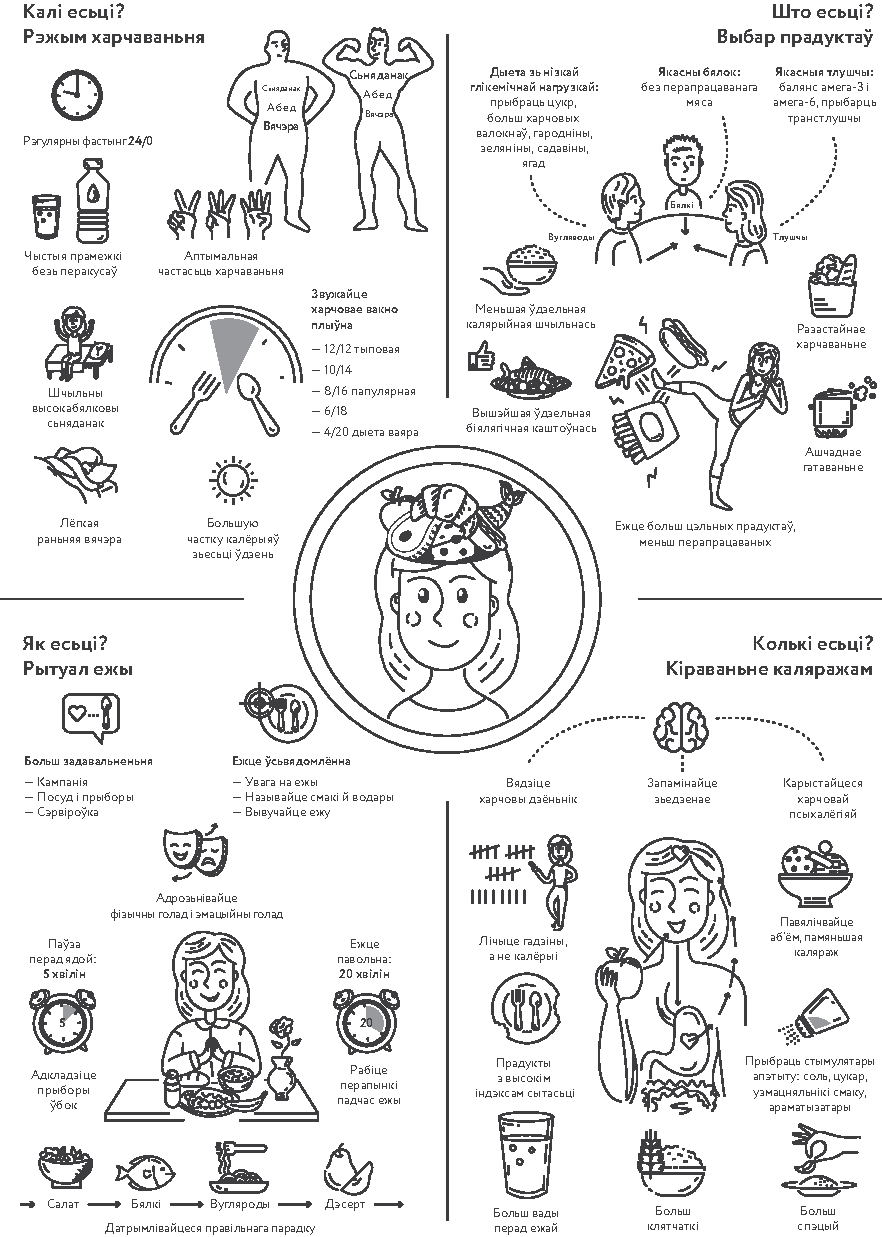
\includegraphics[width=\textwidth]{willpower/ch4/full.pdf}  
\end{figure*}

